\chapter{Results} \label{chapter-results}

The two main hypotheses of this thesis are, first, that the financial sector affects the ownership of housing and therefore the class structure of society, and, second, that this may have implications for urban productivity.  In this chapter, we present model results relevant to these hypotheses.

In the first part of this chapter, we describe the results from the model with no policy interventions. In the second part, we explore the effects of six policy interventions without the link from housing to productivity. In the third part, we repeat the six policy interventions with the link from housing to productivity.  %33\% % With the link, increased rates of financialized ownership reduce the value of the production parameter $A$. 
In the fourth section, we present the results with and without productivity impacts side-by-side. {\color{red} ADD SHOCK SECTION} This makes it easier to compare the effect of policies with and without the productivity linkage. 

The policy variables we consider are: 
\begin{enumerate}
\item Capital gains taxes, which capture part or all of the speculative gains on property ownership. Raising them does not affect the use value of a property, but should make the property less attractive to speculators and reduce the amount owner-occupiers will bid. 
\item The cost of capital, or the rate at which investors can borrow, which affects the net return to property speculation.
\item Transportation costs, which are affected by public infrastructure investment, reduce the amount of locational value that is spent on transportation, increasing the wealth of the community 
\item Urban density, which is controlled by zoning regulation, and which multiplies locational rents. 
\item The sensitivity of the cost of borrowing to borrower wealth, which affects whether low-asset households can purchase housing and the likelihood they will service mortgages.
\item The property tax rate, which is a cost of living in the city. The tax is deducted from locational rents for individuals or speculators.
\end{enumerate}
Because there are multiple effects of each intervention, we use separate figures to represent the impact of each policy intervention on the trajectory of each of the seven indicator variables. %In the absence of linkages between the housing market and the production sector we see population effects but no effect on firm variables wage, capital stock or workforce. This is because we force the number of firms to accommodate increases in population. Different assumptions will allow growth in both firm size and number, but we are not interested in short-term firm dynamics, and the case we consider is easier to interpret. 
The variables we consider are:
\begin{enumerate}
    \item Wage levels
    \item Capital stock
    \item The size of the firm workforce
    \item Total employment
    \item City extent
    \item Number of firms and 
    \item The share of owner-occupants in the workforce
\end{enumerate} 
In total, there are forty-two plots in the first section, some showing a null effect. There are an additional forty-two plots in the second section. We discuss each experiment, point out the most significant effects, and provide some explanation of results that may seem surprising.  


These results are conditioned on the selection of the parameters of the model. We choose parameter values to approximate those for a mid-sized city so the results may be more easily interpreted.  The size of the effect will vary if different parameters are chosen. % However the qualitative results are not affected by small variations in parameters. 
% It is important to remember that the results we report are qualitative, not quantitative results. 
%First we will explore the impact of financialization on productivity we will introduce explicit links between ownership and productivity in Chapter~\ref{chapter-tramsmission}
%We are currently observing these processes underway in the real world. We need to know if they are explained by a theoretically-consistent model of the urban economy that incorporates the financialization process.
For the experiments, we test relatively large perturbations of the parameters to make the effects of interventions clear. Appendix~\ref{appendix-parameters} documents the parameter values.


Since the purpose of this model is \gls{theoretical exposition}, the results are the results of explorations within the model and we make no claims about the outside world. % based on the results generated for the model. 
The results are simply the output, given the relationships in the model. 
Without strong empirical support for parameter values, we can say little about the magnitudes of any effects, although we can have some confidence in the directions and relative sizes.  Further experiments would be needed to nuance the relationship between the variable in the model and output and extensive empirical work would be needed to make any specific claim about the outside world. 
The results may, however, suggest questions, hypotheses or topics for future work. % We've made the case that these questions matter given the process of financialization underway in cities. 


% We illustrate dramatic policy changes and strong productivity linkages to ensure the qualitative impacts are easy to identify. 




\section{The basic ownership result}


\begin{figure}
\centering
\begin{tikzpicture}
\draw [fill=yellow!15] (-1.7,1)--(1.7,1)--(3,5.7)--(-3,5.7)--cycle;
  \node[text width=4.5cm, align=center] at (0,0) (1) {\textbf{Urban structure and production sector}};
   \node[above=-1mm of 1] (A1) {$\uparrow$};
   \node[above=1mm of A1] (Pop) {Population};
   \node[above=-1mm of Pop] (APop) {$\uparrow$};
   \node[above=-1mm of APop]  (3) {Bids};
   \node[above=-1mm of 3] (4) {$\uparrow$};
   \node[above=-1mm of 4] (5) {Ownership};
   \node[above=-1mm of 5] (6) {$\uparrow$};
   \node[above=-1mm of 6] (7) {Rent distribution};
   \node[above=-1mm of 7] (ARent) {$\uparrow$};
    \node [above=1.2mm of ARent, text width= 7cm, text centered] {\textbf{}{Growing inequality\\Tenant sojourner cities\\ Eviction of families from cities\\ End of urban home-owning class}};

   % \node[above=1mm of 1] (2) {$\uparrow$};
   % \node[above=1mm of 2] (3) {Growing inequality};
   % \node[above=1mm of 3] (4) {$\uparrow$};
   % \node[above=1mm of 4] (5) {Eviction of families from cities};
   % \node[above=1mm of 5] (6) {$\uparrow$};
   % \node[above=1mm of 6] (7) {Tenant sojourner cities};
\end{tikzpicture}
\caption{The platform, the process, and the outcomes.}
\label{fig:outcomes}
\end{figure}

{\color{red}

REWRITE THIS SECTION 
% Here's the trajectory of how the housing market is changing.

% Here's the result of the changes in ownership
% Here's what we see with the ownership pattern in the model.

% Sumarize the process of financialisation - not about a figure, what we're talking in this sicture.
% PLEASE SUMARIZE IT FIRST. 



We are running the model and getting results about how the process we observe, build it into the model, and see how the pattern of ownership changes, and we see the results of that. We see the changes in ownership based on this process running through the model.

When we run the model with no parameter interventions, we see a steady rise in financialized ownership. 

The model we've built is an attempt to build a theoretical model of a process like what we observe happening in the financialization of cities. Figure~\ref{fig:outcomes} summarizes the process that we observe happening in cities, and have attempted to model. Financialization claims an increasing share of rents in the cities. % we have explained in previous chapters. 
At the bottom of the figure, the \gls{Alonso-Jacobs model} produces demand for land and drives population. In the housing market section, agents bid for land. Competition between would-be owner-occupiers and investors results in an evolving allocation of ownership of land. Within the model, properties are put up for sale, financial actors purchase an increasing number because they have advantages over private buyers. Primarily these advantages are related to increased ability to access capital and are based on realistic parameter values. The results are growing inequality, eviction and the loss of an urban class of home-owners, capturing and holding assets in the urban center. % The behaviours of the model agents combine to produce the results at the top of Figure~\ref{fig:outcomes}. 

\begin{figure}[h!tb]
    \centering
    \hspace{4cm} % Adjust the amount of space as needed
    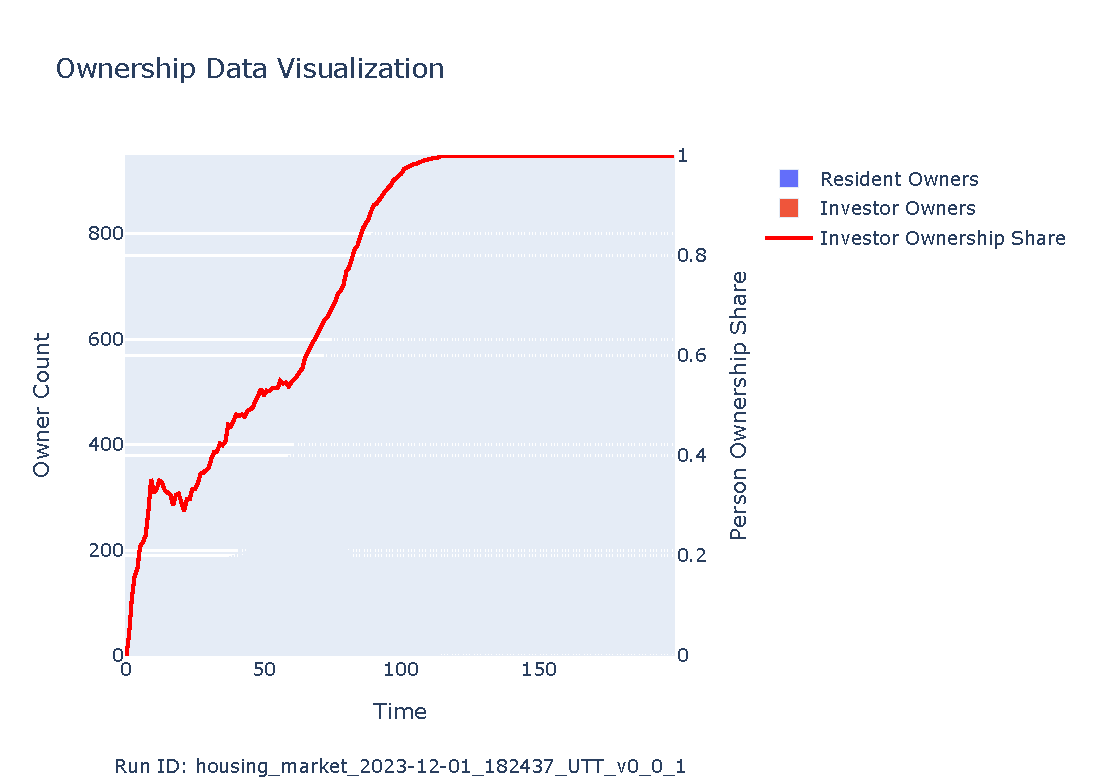
\includegraphics[scale=0.8, trim={0 1cm 0 1.8cm}, clip]{fig/Analysis/Ownership_Data_1.pdf}
    \caption{The transformation from a city of homeowners to a city of tenants in the baseline model.}
    \label{fig:Baseline_ownership_trajectory}
\end{figure}


% Before presenting the results, we briefly review how they arise and how the key ownership results are presented. 
Figure ~\ref{fig:Baseline_ownership_trajectory} illustrates the basic ownership result of the model. It depicts the evolution of the housing market using a version of the model that grows over 200 years from 50 homeowners to a population of 1,000. The number of homeowners is shown by vertical blue bars.  Red bars show counts of investor-owners and the solid red line shows the share. (In the rest of this chapter we report only shares.) 
At first, there are no investor-owned homes, shown by red bars. The number of owner-occupiers initially rises faster than the number of investors, but after one hundred periods it falls to zero. Investors eventually own all of the housing in this example. 
 
The red line, with its scale on the right of the figure, shows the share of the housing stock owned by investors. By the time the city reaches its maximum size, the city has been transformed from a city of homeowners to a city of tenants. The erratic rise of the red line appears to signal a transitional range in which investors and would-be owner-occupiers are similar in number and competitive strength. In that range, randomness in the savings of new entrants affects the number of units going to each type of buyer. 

With plausible parameter settings, our model consistently produces trajectories similar to this example. We conclude that without countervailing forces, financial actors will take an increasing share of ownership in the housing market. 
%The pattern of ownership established this way determines how locational rents within the city are distributed. %The consequences of any shift from owner-occupancy to tenancy, shown in red, are dramatic. 
%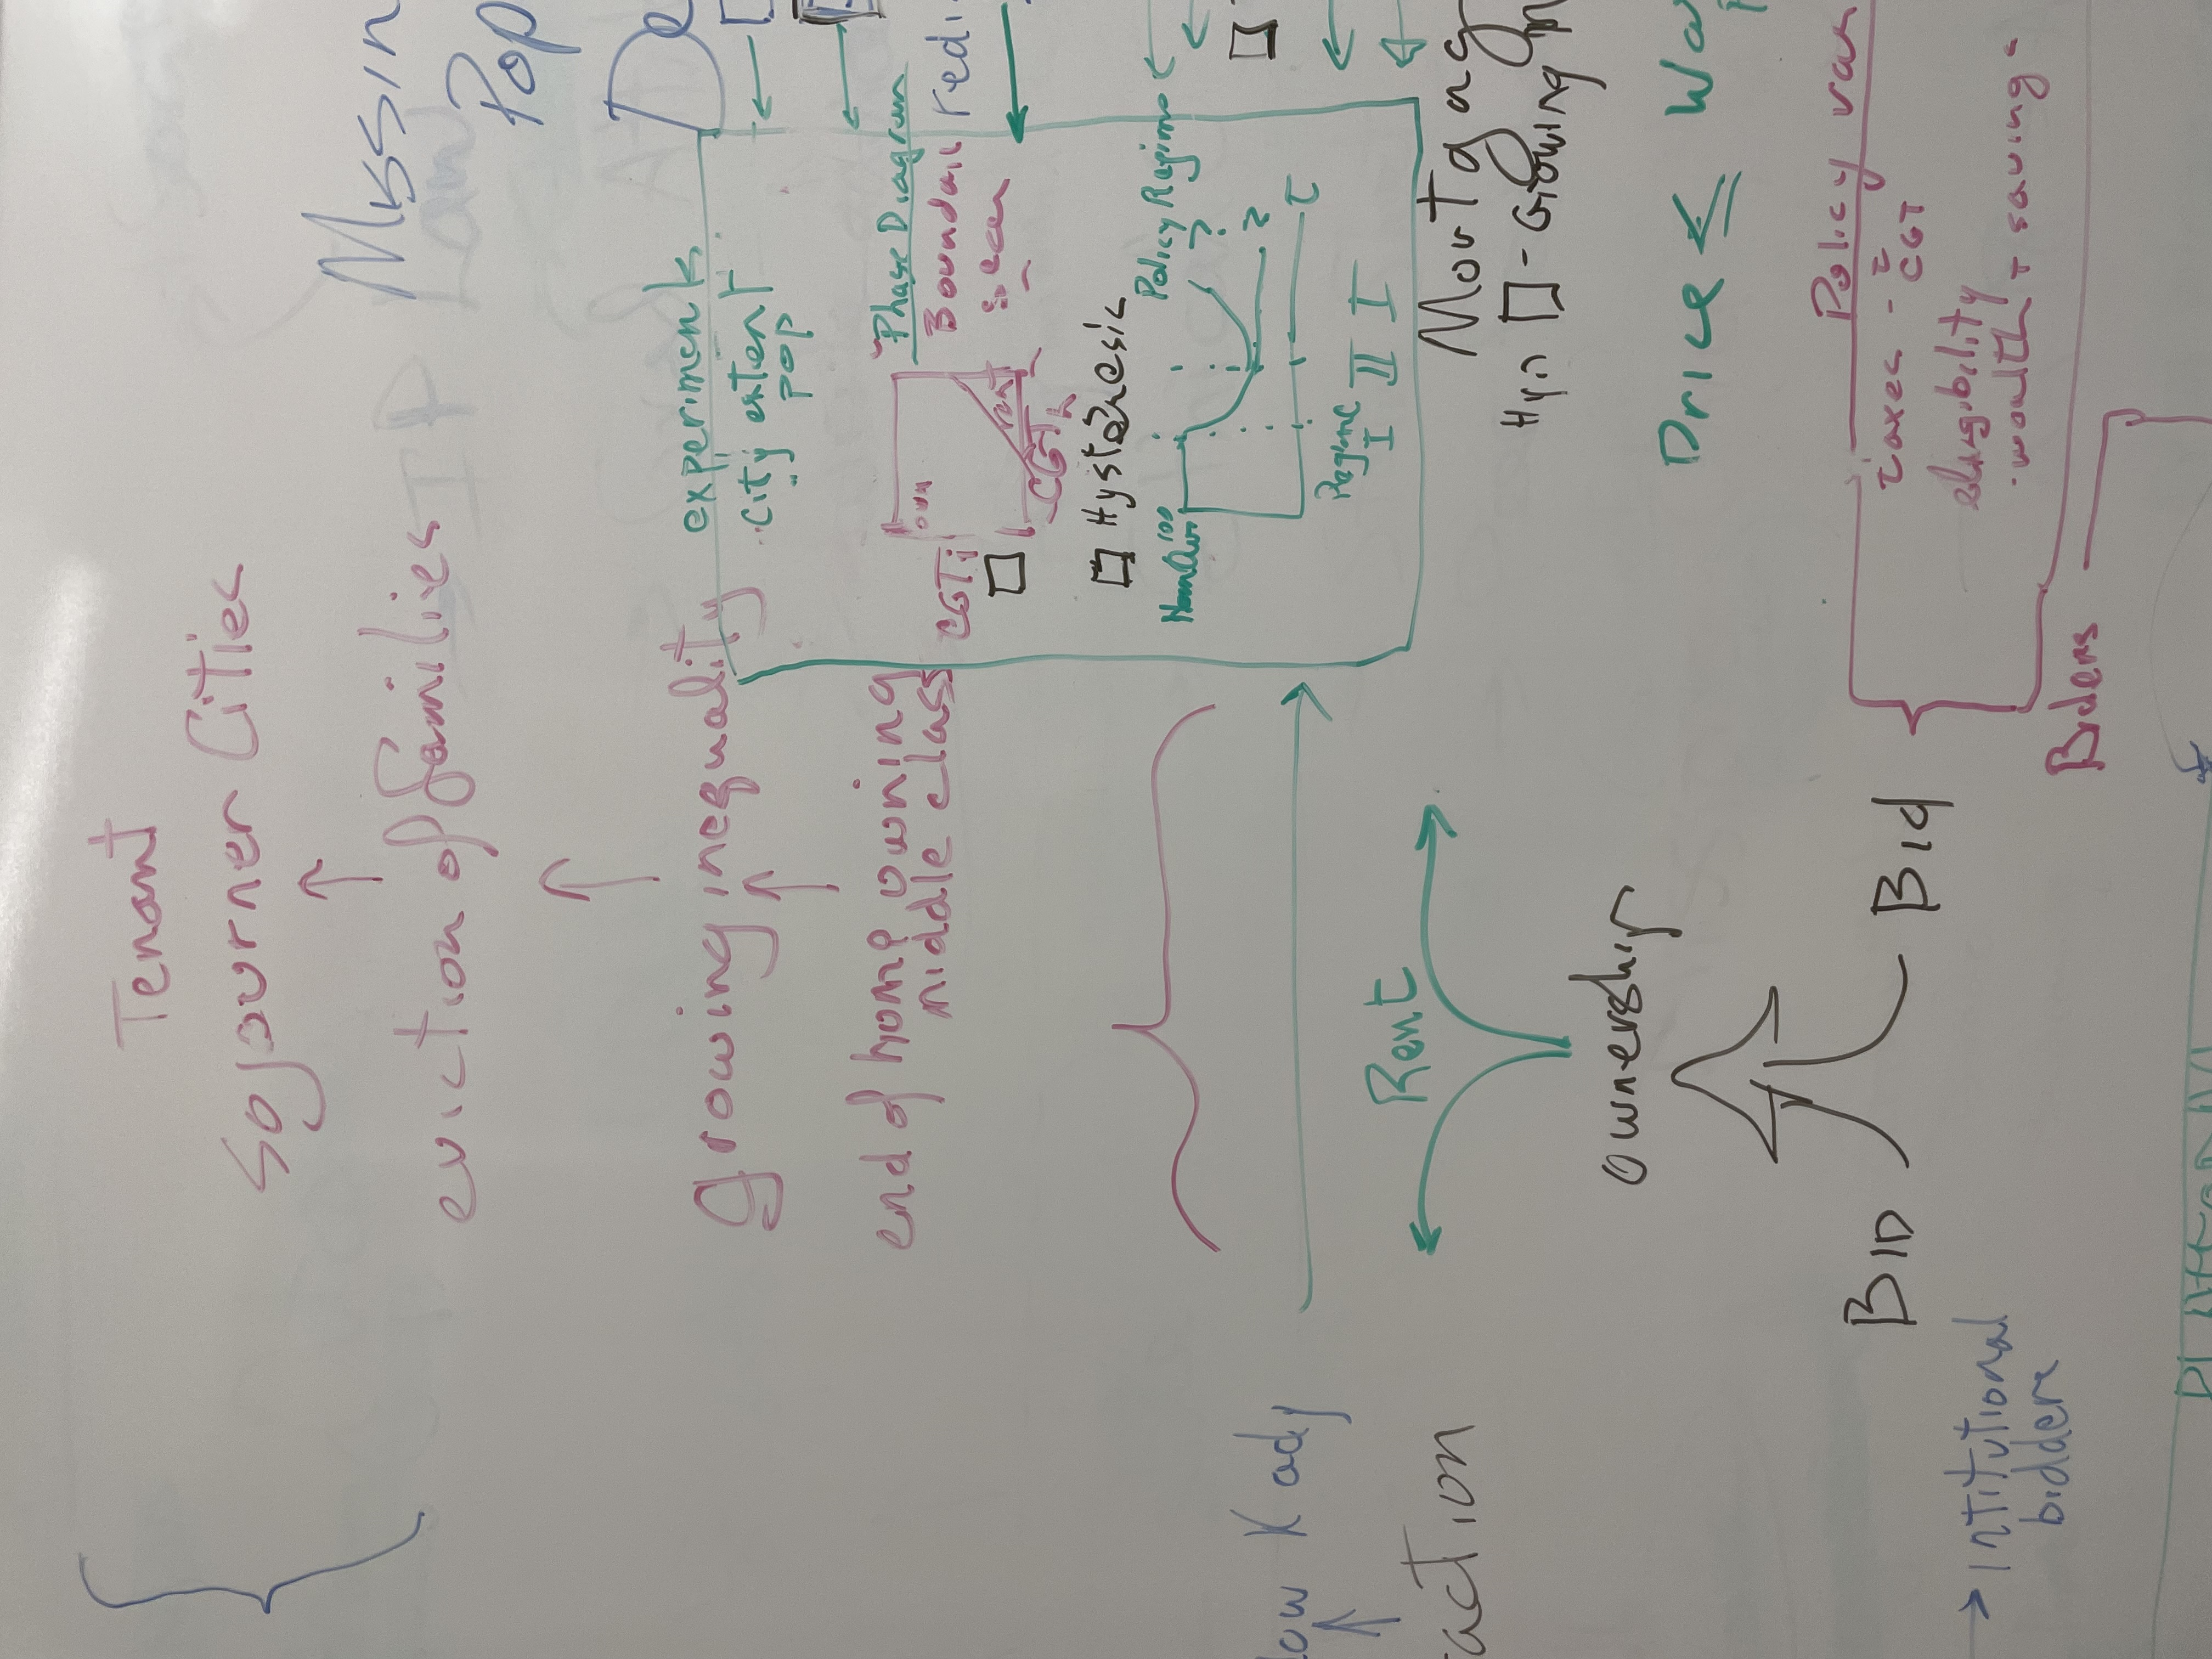
\includegraphics[scale=.5, angle=-90]{fig/IMG_2691.jpg}
The distribution of ownership determines the distribution of the locational land rents, which are the product of agglomeration effects. 

The tendency for investors to own an increasing share of the housing stock is robust in our model. 
Initially, 100\% of locational land rent accrues to residents.   Annual locational rents at the end of the period of growth are approximately twenty times their initial size. At that point 100\% accrues to the owners of financial capital. %\footnote{Recall that the radius of a circular city is proportional to the wage premium. Rent can be visualized as a cone of volume $\pi r^2 h/3$ where $h$ is the wage premium. If we double $h$, the volume is increased by a factor of 8.}

}

\section{Policy interventions without productivity link}


This section examines seven potential policy interventions and their effects on ownership. In each case we vary one  variable that can be affected by public policy and examine how the city's evolution is affected.


\newpage

\begin{figure}[]
    \centering
    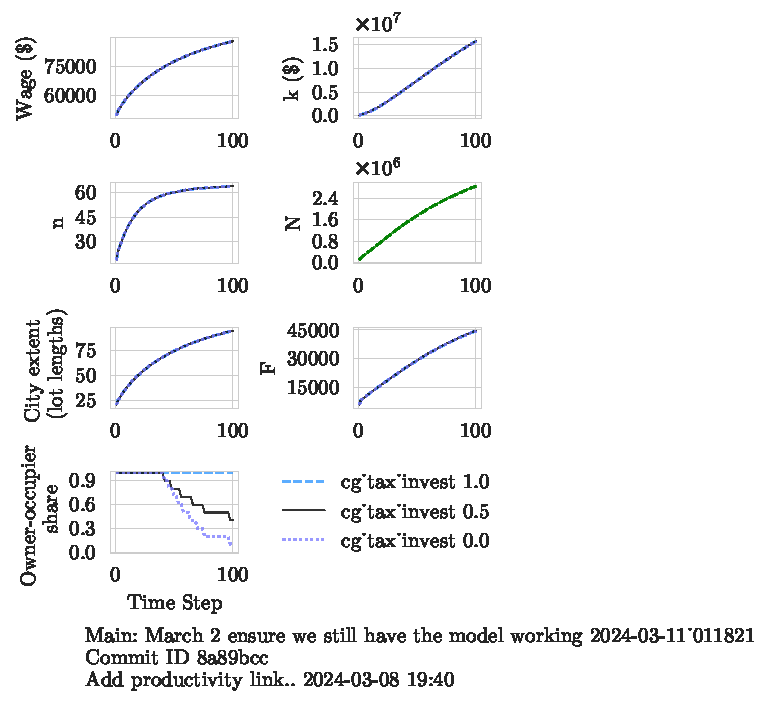
\includegraphics[scale=1.2, trim={0 1.4cm 4cm 0},clip]{fig/cg_tax_invest-Main-011821.pdf}
    \caption{The effect of a capital gains tax on investors.}
    \label{fig:CGinvest_ownership_trajectory}
\end{figure}

\subsection{Capital gains taxation on investors}

A \gls{capital gains tax} is a tax on profit from the sale of property or an investment. It captures the increase in the price of an asset due to changes in the market rather than any increase in value contributed by the owner. The Canadian capital gains tax rate is lower than the tax on interest or dividend income so capital gains are an especially attractive form of income for investors.

In this experiment, we introduce capital gains tax specifically for investors, which we define as any home owner who does not occupy the housing unit. If capital gains are part of the objective of investors, a capital gains tax will, in theory at least, reduce investor participation. Figure~\ref{fig:CGinvest_ownership_trajectory} shows this is the case. A capital gains tax on housing investment will have a powerful effect on the ownership ratio but not affect other variables. The result was achieved in a situation where homeowners do not pay a capital gains tax when they sell. 

\newpage

\subsection{Capital gains tax on owner-occupiers}

\begin{figure}[b!]
    \centering
    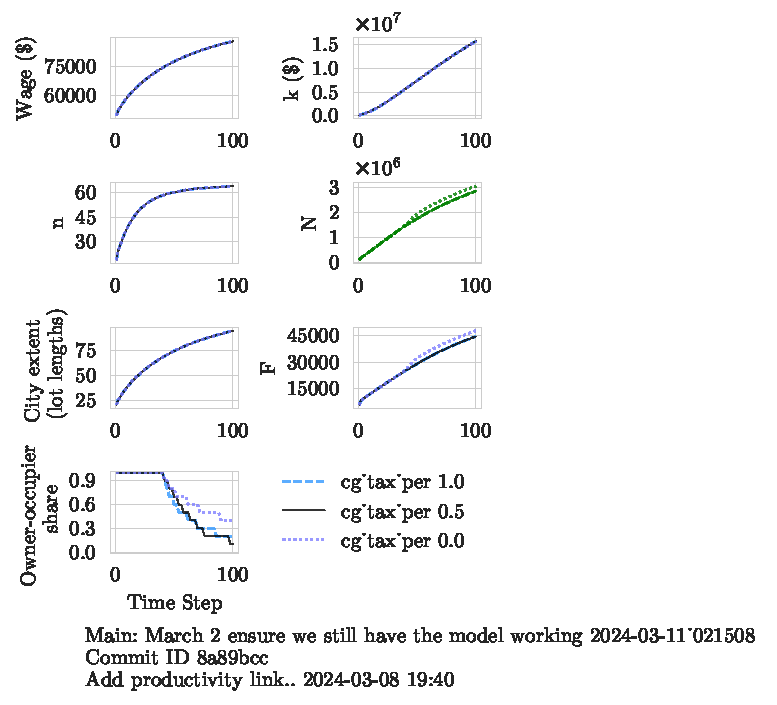
\includegraphics[scale=1.2, trim={0 1.4cm 0 0},clip]{fig/cg_tax_per-Main-021508.pdf}
    \caption{The effect of a capital gains tax on homeowners. The dotted line represents the case with no capital gains tax for homeowners.}
    \label{fig:CGpers_ownership_trajectory}
\end{figure}

In Canada, homeowners currently do not pay capital gains taxes on their primary residence. This is a policy that has been questioned because it favours owners over renters whose investments would be subject to taxes. Figure ~\ref{fig:CGpers_ownership_trajectory} shows of the effect three different  capital gains tax rates, 0\%, 50\% and 100\% on owner-occupiers. The capital gains tax rate for investors in this set of experiments is 15\%. In both of the cases with  the owner-occupiers' tax rate  higher than the rate for investors, %, shown by the solid and the dashed lines,  
home ownership falls dramatically. Reducing the capital gains for owners makes purchasing a home less attractive as an investment owner occupiers but not for non-resident owners. Rents do not fall for tenants in our mode, however. Landlords continue to charge tenants the full locational value and the locational value does not depend on whether there are capital gains for property owners. 

In this case, the capital gains tax on investors is set at 15\%. {\color{red} ALSO GIVE VALUES FOR OWNER OCCUPIERS - ALSO IS IT WEIRD THAT WE HAVE INVESTOR AT .15 AND THEN ONLY TEST FOR OWNER OCCUPIERS AT 1. .5 AND 0? MAYBE JUSTIFY A BIT MORE}
 



%%%%%%%%%%%%%
%\newpage

\subsection{The cost of capital for investors}

% 'r_investor': [0.2, 0.1, .05] has set up for morning
The cost of capital is the interest rate on borrowed money. Higher capital costs for investors might be expected to slow the rate of housing acquisition because it makes acquiring housing more expensive for them. Figure ~\ref{fig:capital_ownership_trajectory} shows the effect of increasing capital costs for investors. Surprisingly, higher capital costs appears to increase the speed at which investors purchase but it does not affect the final level of investor ownership.  In addition, it appears to decrease population, suggesting that the cost of acquiring housing to live in rises. The cost of capital for investors is not an obvious policy tool, so we don't think this result is of great interest politically, but it warrants further study.

{\color{red} CHECK THIS--RERUN. THIS RESULT DOESN'T REALLY MAKE SENSE.}

\begin{figure}[h!t]
    \centering
    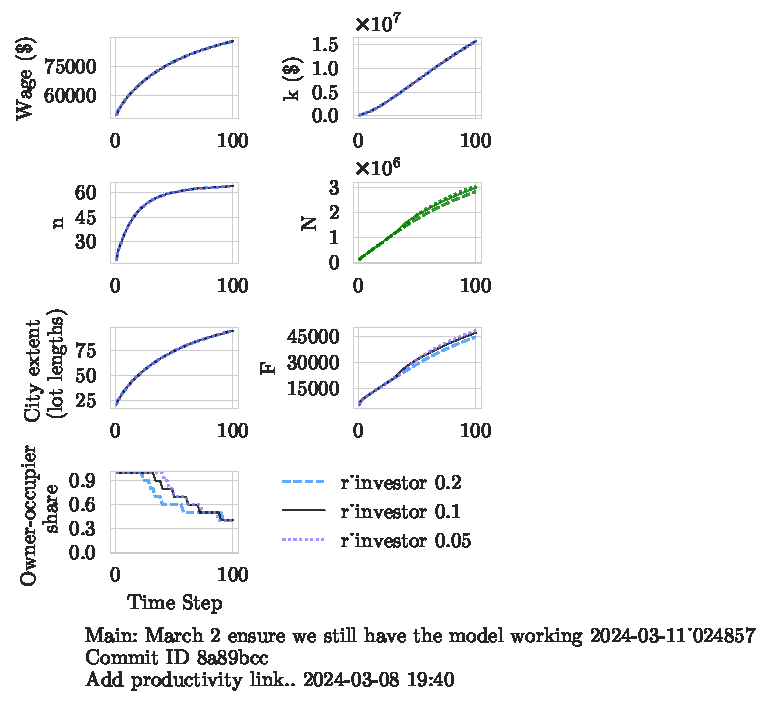
\includegraphics[scale=1., trim={0 1.4cm 0 0},clip]{fig/r_investor-Main-024857.pdf}
    \caption{The effect of raising capital costs}
    \label{fig:capital_ownership_trajectory}
\end{figure}

\newpage
\subsection{Transportation costs}
Roads and managing road congestion, as well as the transit system are public responsibilities that affect the cost of transportation. % Can reducing the cost of transportation affect the ownership ratio? 
Figure~\ref{fig:c_ownership_trajectory}, shows the results of reducing transportation costs for everyone by 40\%. 
%This is what we expect in the Alonzo model within this model.
We expected the city would grow faster and get larger with lower transportation costs. This effect was indeed observed. 
% 'c': [500, 300],

Less obviously, lower transportation costs also served to decrease the home-ownership ratio. The reduction in transportation costs leads to an increase in land rents, and the increase in land rents increases the rate of increase of property prices, leading to higher expected capital gains and ultimately less ownership by owner-occupiers. 

\begin{figure}[h!t]
    \centering
    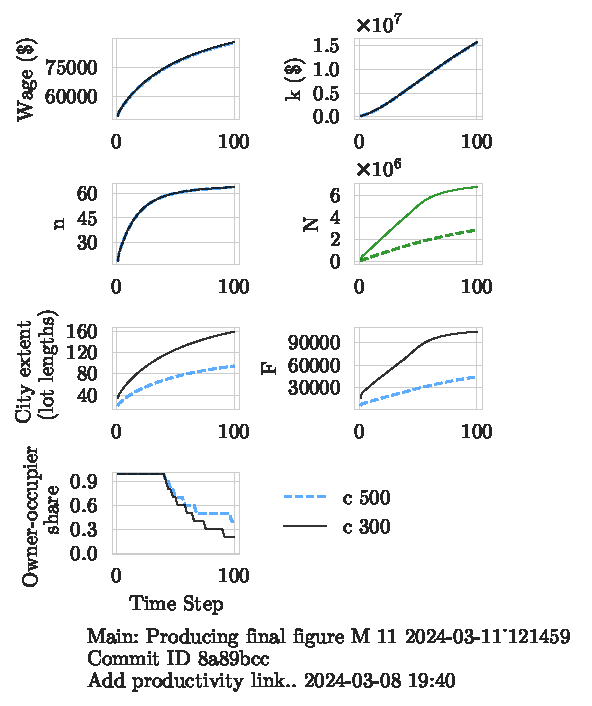
\includegraphics[scale=1, trim={0 1.4cm 0 0},clip]{fig/c-Main-121459.pdf}
    \caption{The effect of decreasing transportation costs}
    \label{fig:c_ownership_trajectory}
\end{figure}

\newpage
\subsection{Density}
% 'density': [100, 150]
% Density is a policy variable that is much discussed. 
Increasing density is proposed as a way to increase housing availability and the ability of people to buy homes. Our results indicate that the effect of density on city population is significant but it has no effect on city extent and no effect on the ownership ratio. The first two results are expected, the third less so, but it is easily explained. 

Figure~\ref{fig:density_ownership_trajectory} shows that the share of homeowners is not affected, only the number of homes is. Since rent per unit is unchanged, density alone does not affect the relative advantage of new home buyers and investors, leaving the ratio constant. There are more homes, however, and, since the ratios are consistent, there are more homeowners. 

\begin{figure}[h!bt]
    \centering
    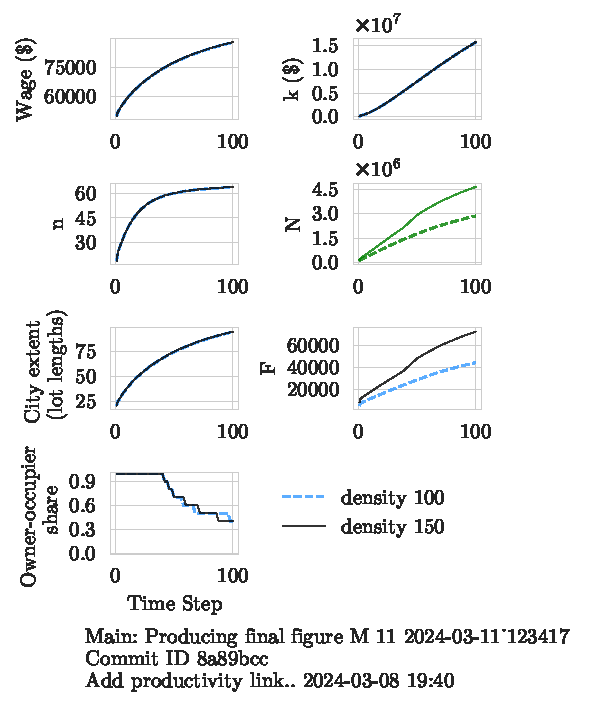
\includegraphics[scale=1, trim={0 1.4cm 0 0},clip]{fig/density-Main-123417.pdf}
    \caption{The effect of increasing density}
    \label{fig:density_ownership_trajectory}
\end{figure}


\newpage
\subsection{Cost of financing's dependence on borrower's wealth}
Wealth sensitivity in our model is a parameter of the banking system. It determines how easy it is for people with limited assets or income to get a mortgage. A higher value is more restrictive,  making it harder for an asset-poor person to get a mortgage.

Figure~\ref{fig:wealth_sensitivity_ownership_trajectory} illustrates that a restrictive mortgage regime slightly reduces the labour supply and city population. It has no noticeable effect on the ownership ratio. Since the purpose of a restrictive policy is to reduce defaults and bankruptcies, the small impact on other variables suggests that as a policy it can be adopted without needing to consider the economic impacts on the city. 
% 'wealth_sensitivity': [0.15, 0.1, 0.5]

\begin{figure}[h!bt]
    \centering
    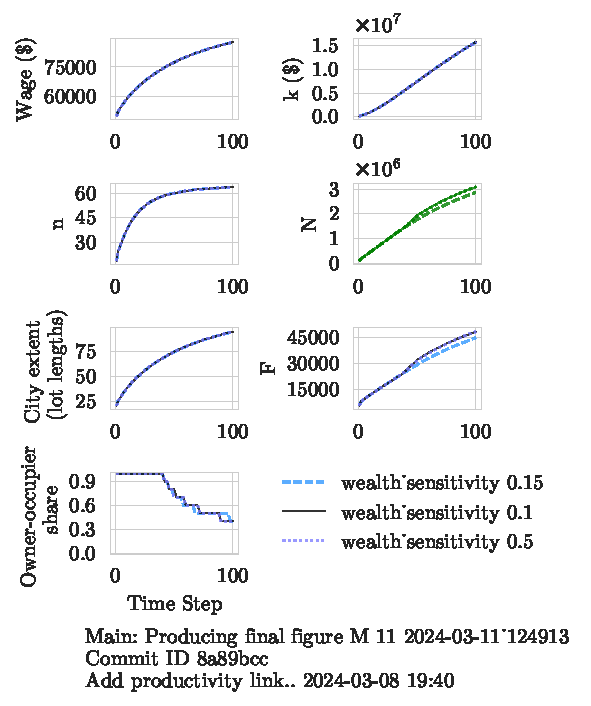
\includegraphics[scale=1, trim={0 1.4cm 0 0},clip]{fig/wealth_sensitivity-124913.pdf}
    \caption{The effect of wealth sensitivity of mortgage access}
    \label{fig:wealth_sensitivity_ownership_trajectory}
\end{figure}

\newpage
\subsection{The property tax rate}
{\color{red} ADD SOMETHING ABOUT THE RESULTS .. Figure~\ref{fig:property_tax_ownership_trajectory} shows ...}\footnote{The property tax rate variable is a matter for policy debate because there are good reasons to think, first, that property taxes are a barrier to ownership, and second, that the property taxes are not paying all the costs of public infrastructure and services to homeowners, leading to significant inequities.}

% 'property_tax_rate': [0.1, 0.05, .01] k doing}
\begin{figure}[h!tb]
    \centering
    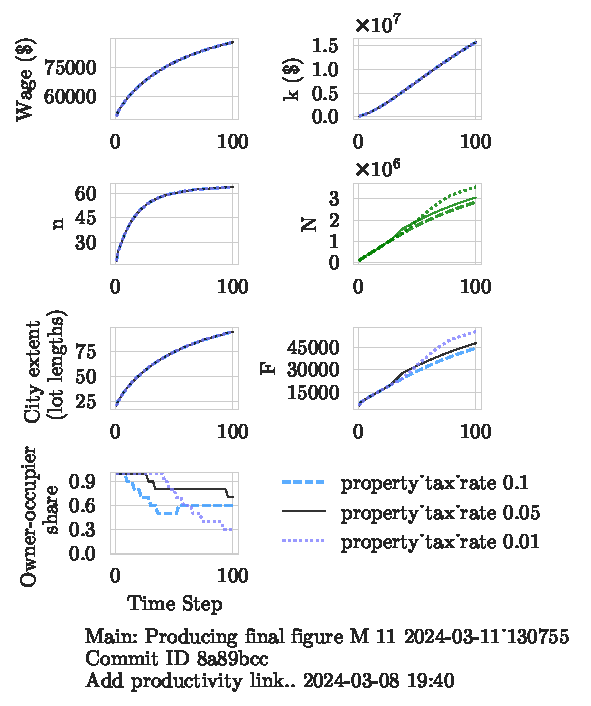
\includegraphics[scale=1.1, trim={0 1.4cm 0 0},clip]{fig/property_tax_rate-Main-130755.pdf}
    \caption{The effect of property tax rates}
    \label{fig:property_tax_ownership_trajectory}
\end{figure}




\newpage
\section{Policy interventions with a productivity link}


We have a hypothesis that there's a link to productivity, if there is such a link, we want to see the implication.
To explore the implications of this link, we've added a link and looked at the implication. 


In this section we explore the effect on the variables we are looking at if this productivity exists. 

{\color{red} WHY A 33\% LINK?}
% In this section, we use our model to explore some implications of a  link between the financialization of an urban housing market and the urban production economy.

In order to capture the link between productivity in output described in Chapter~\ref{chapter-tramsmission}, we model a hypothetical link and consider the effect of the policy interventions with these links in place. We model that link with a relationship where ownership rate affects the parameter $A$ in the firm production function. the 
multiplicative constant term in the Cobb-Douglas and scaling functions. 
% What is the policy effect when there is a link, and we model the link as a change in $A$. 
We repeat the seven policy interventions with the %a 33\% 
reduction in $A$, to understand the implication in the model from introducing the linkage. 
% We will repeat the seven policy interventions with a 33\% reduction in $A$.  
As before, we use separate figures to represent the impact of each policy intervention on the trajectory of each of the seven variables. 

\begin{figure}[h!tb]\label{fig-impact-channel-example}
    \centering
    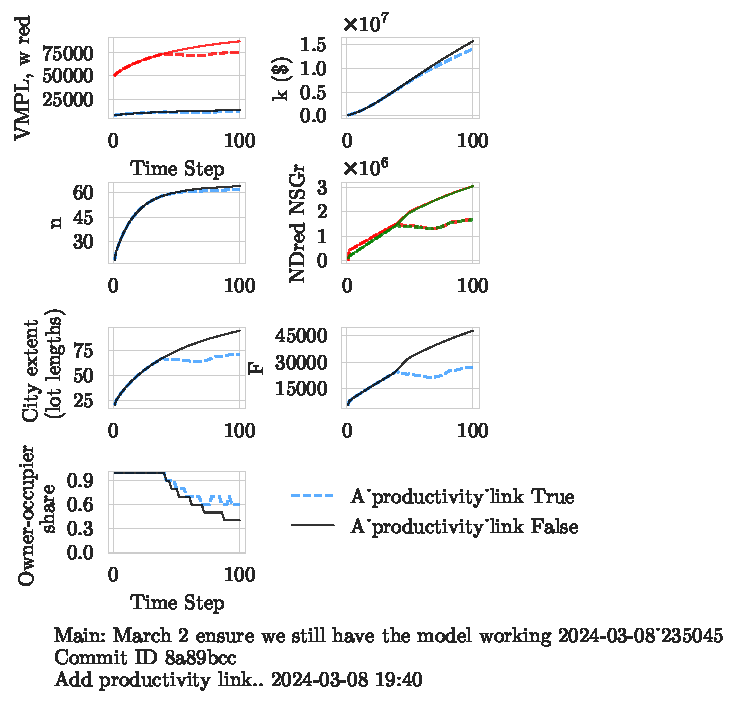
\includegraphics[scale=1, trim=.25cm 2cm .25cm .25cm, clip]{fig/productivity_link.pdf}
    \caption{Illustrating the impact of financialization on an urban economy}
\end{figure}

A simulation of this linkage is illustrated in Figure~\ref{fig-impact-channel-example}. The finance-driven change in ownership share shown in the lower panel transforms a city of homeowners into a city of renters over the course of one lifetime. 
WHAT is A

HOW ARE WE CHANGING IT - A decreases as the ownership changes to some maximum value. 

Given that there is not an established level of change, from the empirical work. we must extametea resonable level for experiment. We choose a change of a third because it is within the range of differences within the range of differences between the value of A--
large impact, in the range of what is a reasonable difference between communities.

We want to see what a big effect, if smaller we'd have to bring it down..

It also reduces the scale parameter {\color{red}WHAT SCALE PARAMETER IS} by a third MEANING---a very large change selected for illustrative purposes. This has, as we hypothesized, substantial economic implications. The change in the class structure of the city induces a decline in worker productivity and capital investment, resulting in reduced firm size, a reduction in the number of firms, and an overall reduction in population. 

Declining productivity is the primary channel for this change, which pulls down the wage and the other population variables. The change is amplified by the resulting reduction in aggregation effects.  If the linkages we have hypothesized exist, the result of financialization would be a poorer society. 


% {\newpage\thispagestyle{empty}
% \vspace{-1.5cm}
\begin{figure}[h!tb]\label{fig-impact-channels2}
%\vspace{-1cm}
\begin{adjustwidth}{-0.24\textwidth}{-0.24\textwidth}
\centering
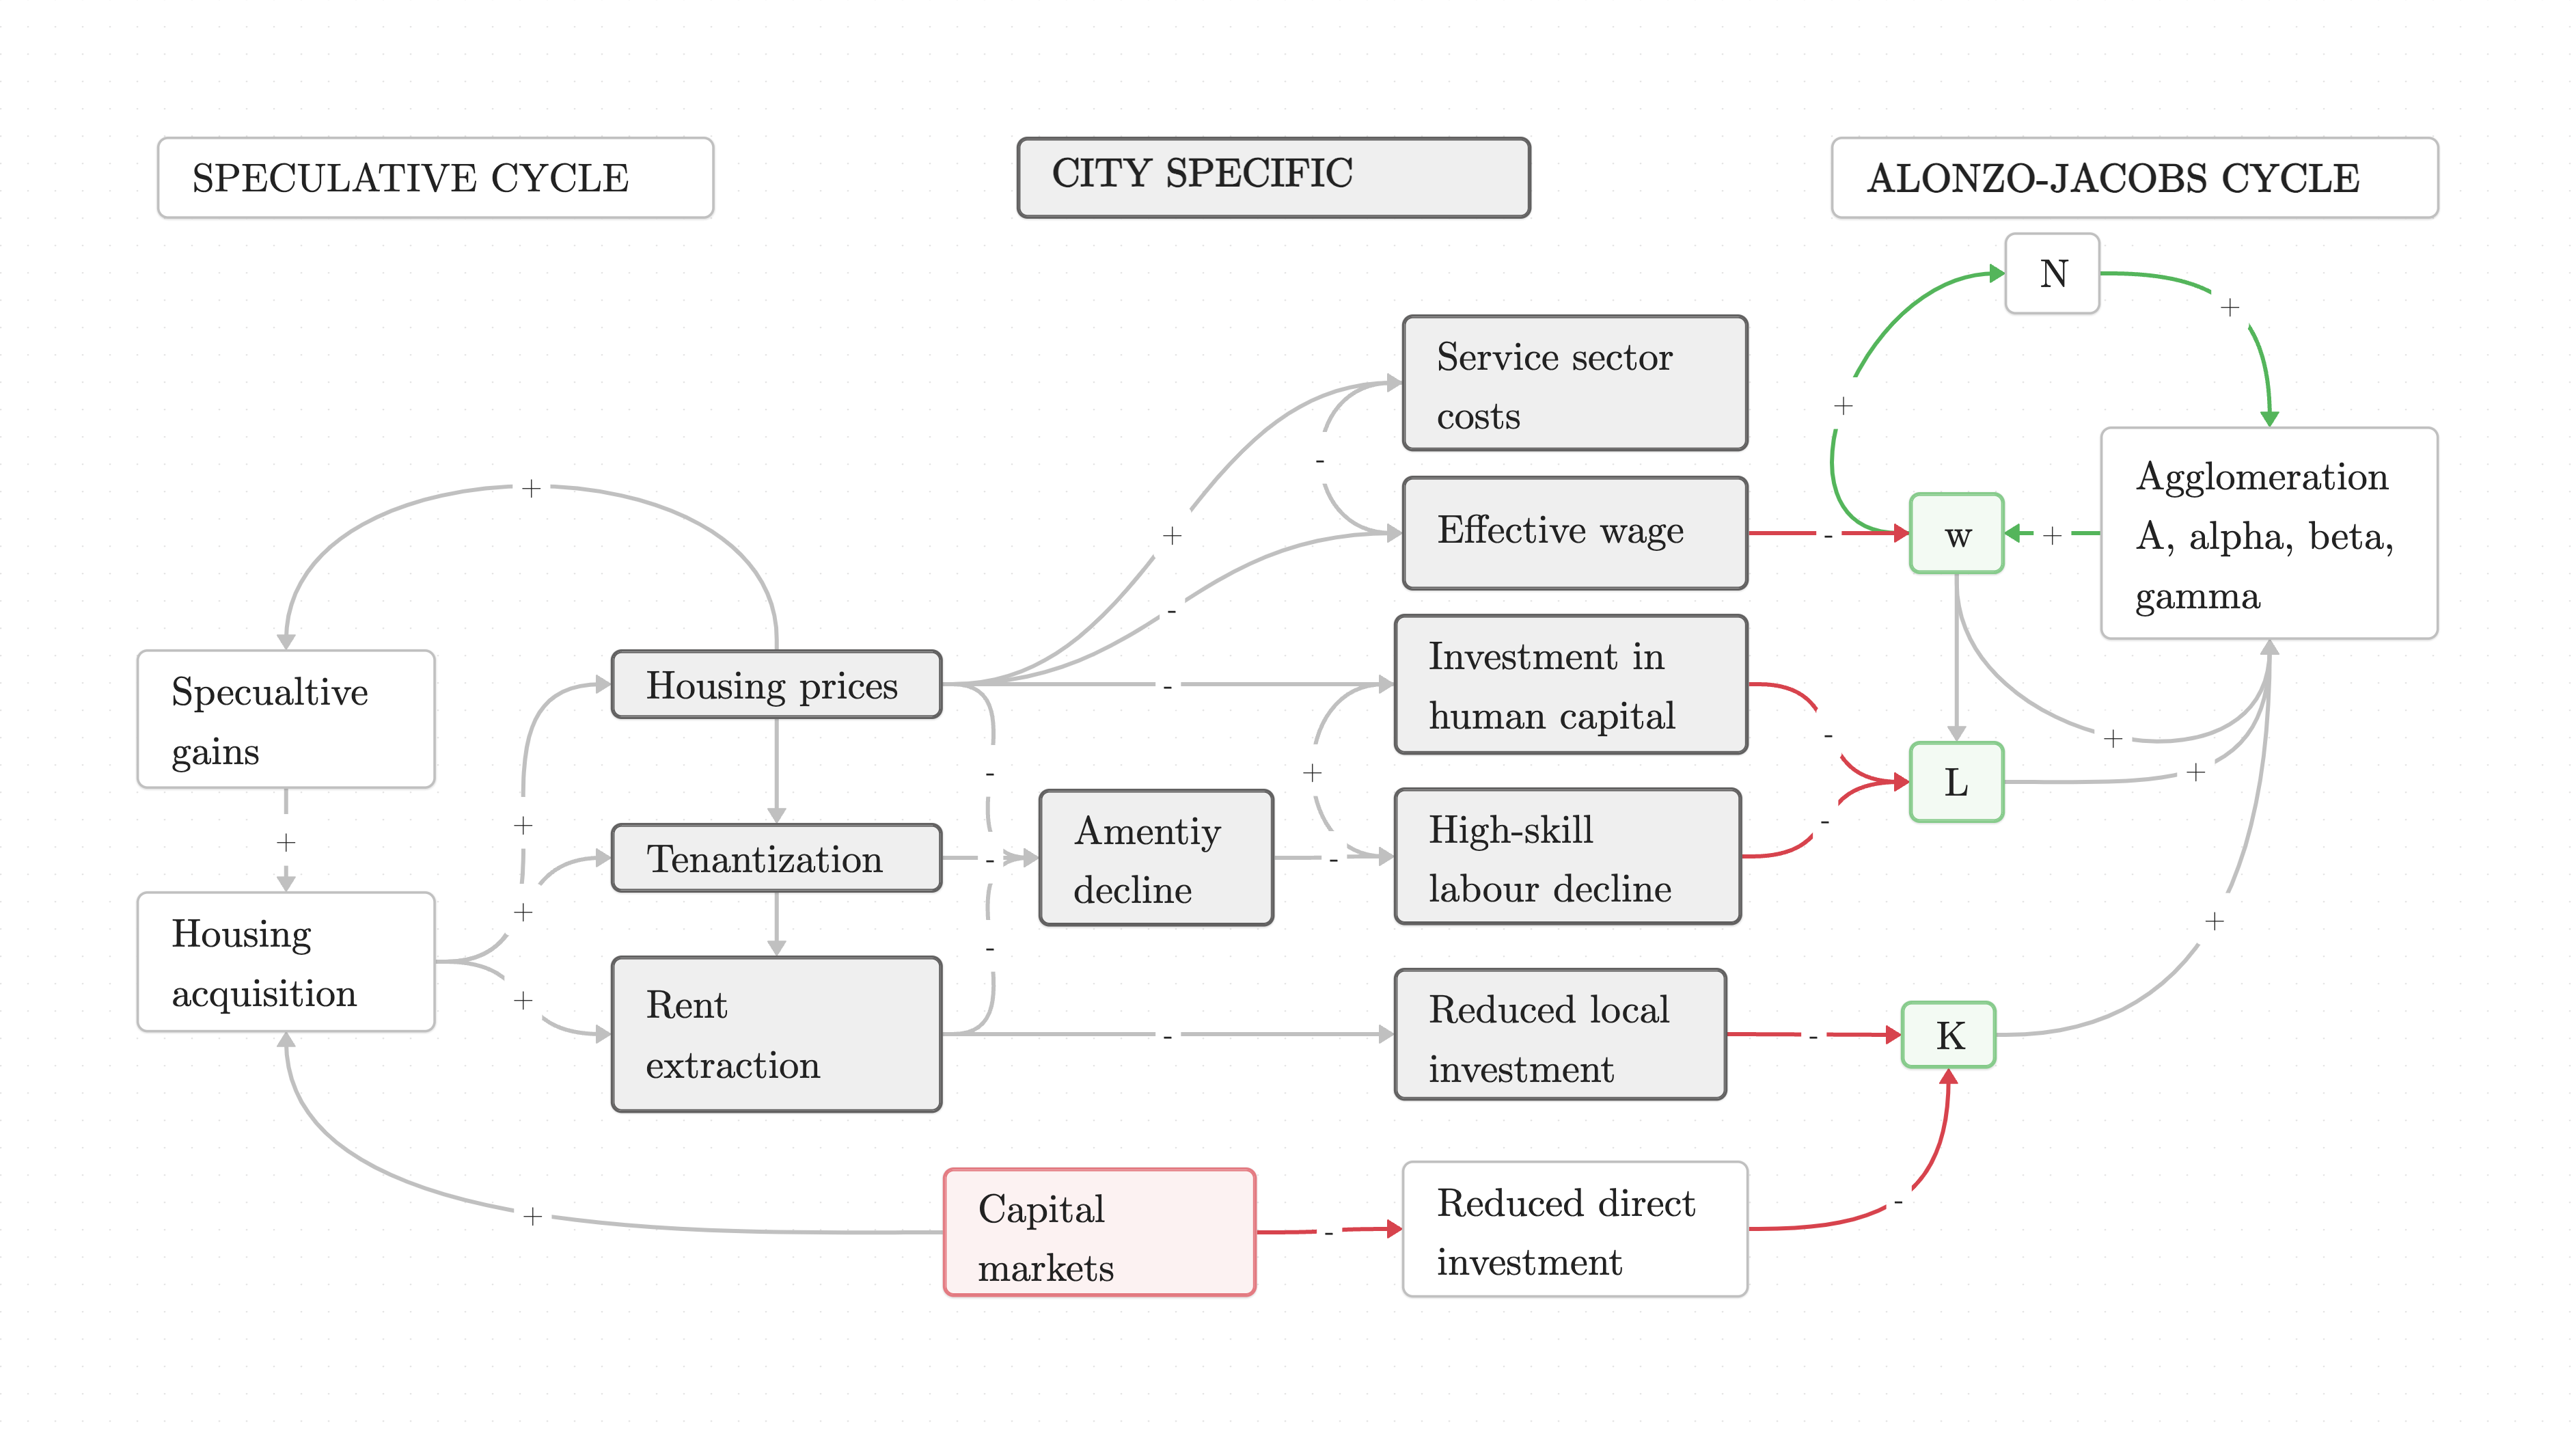
\includegraphics[scale=.15 ]{fig/impact-channels.png}%angle=90
\end{adjustwidth}
\caption{Impact channels relating financialization and urban productivity.}
\end{figure}
%}

This is, to our knowledge, a new result, although it is consistent with fundamental urban theory and with the trends we see today in the urban system. The new component in our result is the formal linkage of the financialized housing market to urban productivity.

We do not have empirical estimates about the strengths of the channels through which the productivity effect would work, however, so only the direction of the impacts illustrated should be taken seriously without further empirical work.  

Assuming there are linkages connecting financialization to productivity, it is important to ask if there are policy implications. 

This experiment indicates that policy parameters are likely to affect the ownership trajectory in different ways when there is a link between financialization and urban productivity and when there is no link.

Figure~\ref{fig-impact-channels2}, repeated from Chapter~\ref{chapter-tramsmission}, showed that while there are many influences on productivity, in our model, they work through specific parameters of the production function, $y=AN^\gamma k^\alpha n^\beta$. 
We chose to illustrate the entire class of linkages by varying the scale parameter $A$, which captures both firm and city-wide effects on productivity. 




\begin{figure}[h!tb] 
    \centering
    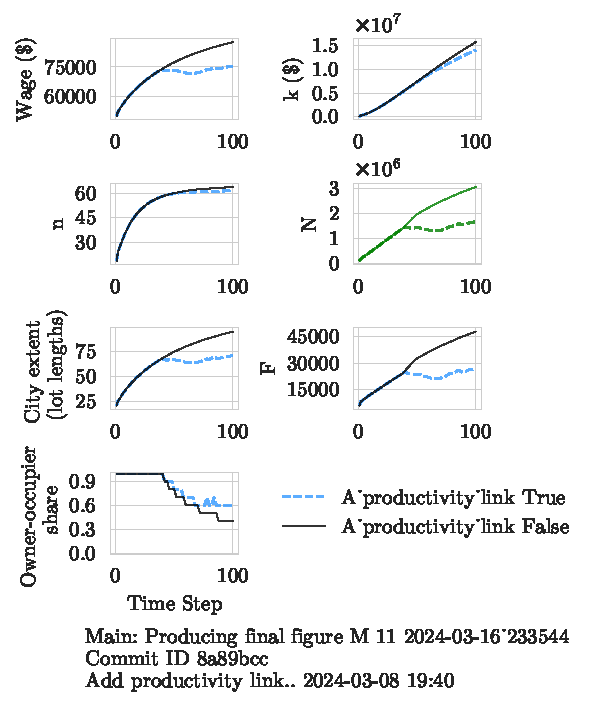
\includegraphics[scale=1, trim={0 1.4cm .8cm 0},clip]{fig/generic-productivity-impact_233544.pdf} 
    \caption{A generic productivity impact associated due to financialization}
    \label{fig:generic-productivity-impact}
\end{figure}

In this section, we will repeat the seven policy interventions with a 33\% reduction in $A$.  As before, we use separate figures to represent the impact of each policy intervention on the trajectory of each of the seven variables. 


\newpage
\subsection{Capital gains taxation on investors}
Figure~\ref{fig-Productivity_link_and_CG} illustrates the effect of increasing the capital gains tax rate on land speculation from 15\% to 100\%  when a link to productivity is present.

\begin{figure}[h!tb]\label{fig-Productivity_link_and_CG}
    \centering
     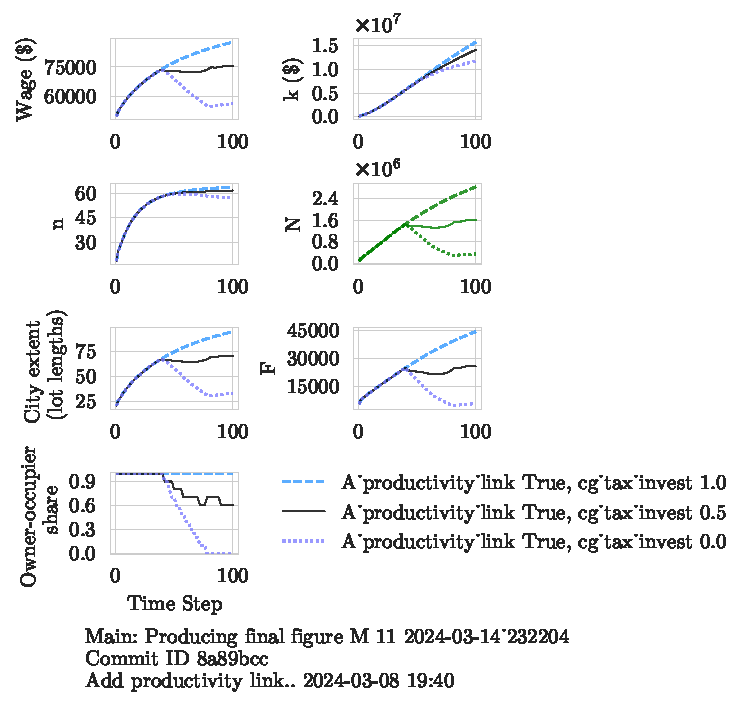
\includegraphics[scale=1, trim=.25cm 2cm .25cm .25cm, clip]{fig/With-productivity_linkcg_tax_invest-232204.pdf}
    \caption{The corrective effect of a capital gains tax with the productivity linkage}
    \label{fig:Productivity_link_and_CG}
\end{figure}

The dashed line in Figure shows that a 100\% capital gains tax on land speculation eliminates investor participation in the market, leaving a population that is 100\%  owner-occupiers whereas without a tax, owner-occupiers are entirely eliminated.  {\color{red} TELL US WHAT IS HAPPENING, NOT WHAT ISNT' HAPPENING} In the absence of taxation on speculative gains, shown by the dotted line, wages are lower, the city is smaller, there are fewer firms and . 

% Wages arehigher, the city is larger, and more firms....
\newpage
\subsection{Capital gains tax on owner occupiers}
{\color{red} MAKE SURE EXPLANATION IS CONSISTENT WITH ABOVE..}

In Figure~\ref{fig:Productivity_link_and_CGpers_ownership_trajectory}, the capital gains tax on investors is set at 15\% and we vary the capital gains tax on owner-occupiers. The dotted line represents the case with no capital gains tax for homeowners. When the tax is higher than the rate for investors, shown by the solid and the dashed lines,  home ownership falls more than in the base case. This case also results in much lower population and city size, which leads to lower rents for tenants because locational rents are lower.

{\color{red}
LOOK AT DIFFERENT VARIABLES WITH THE PRODUCTIVITY LINK..


MAYBE WE ARE MISSING A SECTION RUNNING THE MODEL WITH THE PRODUTIVITUY LINK - MAYBE ON/OFF - BUT WITHOUT ANY INTERVENTION... WE JUST SHOW WHAT HAPPENS IN THE MODEL WITH JUST TURNING PRODUCTIVITY ON

SAY 'THE OWNERSHIP RESULT IS THE SAME, BUT THERE ARE EFFECTS ON THESE OTHER THINGS..'
}

\begin{figure}
    \centering
    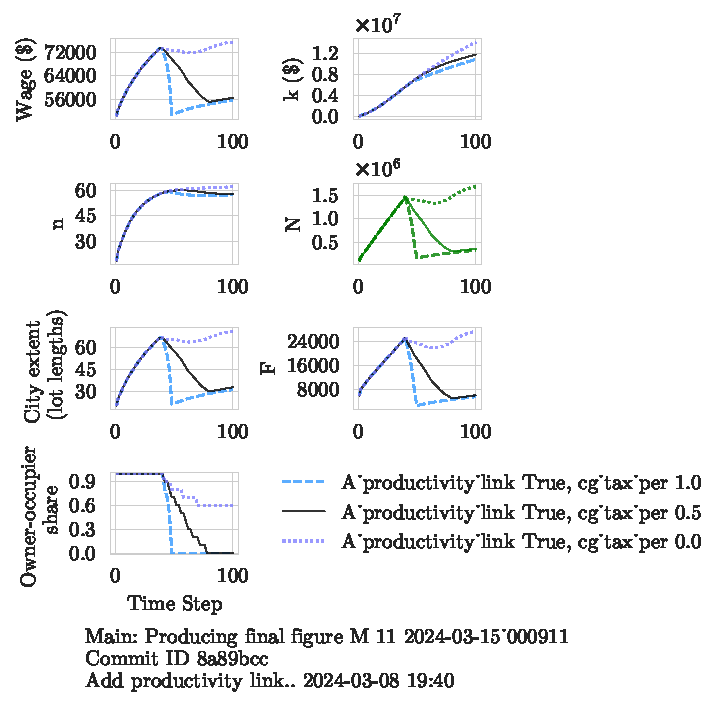
\includegraphics[scale=1, trim={0 1.4cm 0 0},clip]{fig/With-productivity_link_cg_tax_per-000911.pdf}
    \caption{The effect of a capital gains tax on homeowners in the presence of productivity impacts}
    \label{fig:Productivity_link_and_CGpers_ownership_trajectory}
\end{figure}

\newpage
\subsection{The cost of capital for investors}
% 'r_investor': [0.2, 0.1, .05] has set up for morning
Figure ~\ref{fig:Productivity_link_and_capital_ownership_trajectory} shows the effect of increasing capital costs for investors. Even in the presence of strong productivity spillovers, it has little effect, which suggests that the cost of capital for investors does not appear to be a promising policy tool.

\begin{figure}[h!t]
    \centering
   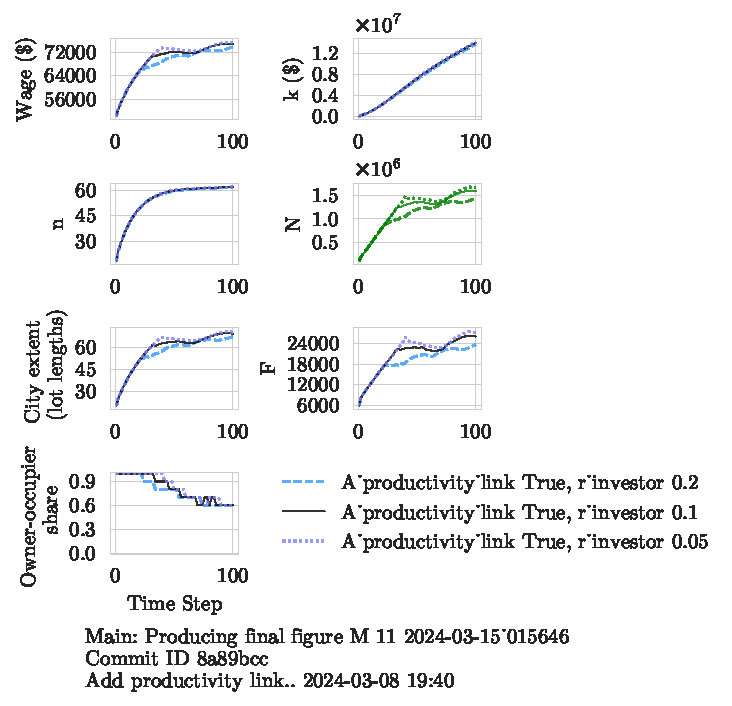
\includegraphics[scale=1, trim={0 1.4cm 0 0},clip]{fig/With-productivity_link-r_investor-15_015646.pdf}
    \caption{The effect of raising capital costs in the presence of productivity impacts}
    \label{fig:Productivity_link_and_capital_ownership_trajectory}
\end{figure}

 
\subsection{Transportation costs}
In Figure~\ref{fig:Productivity_link_and_c_ownership_trajectory}, we reduce transportation costs for everyone. 
Reducing the cost of transportation by 40\% in the presence of productivity impact increases city size and population. 
% 'c': [500, 300],

\begin{figure}[h!t]
    \centering
    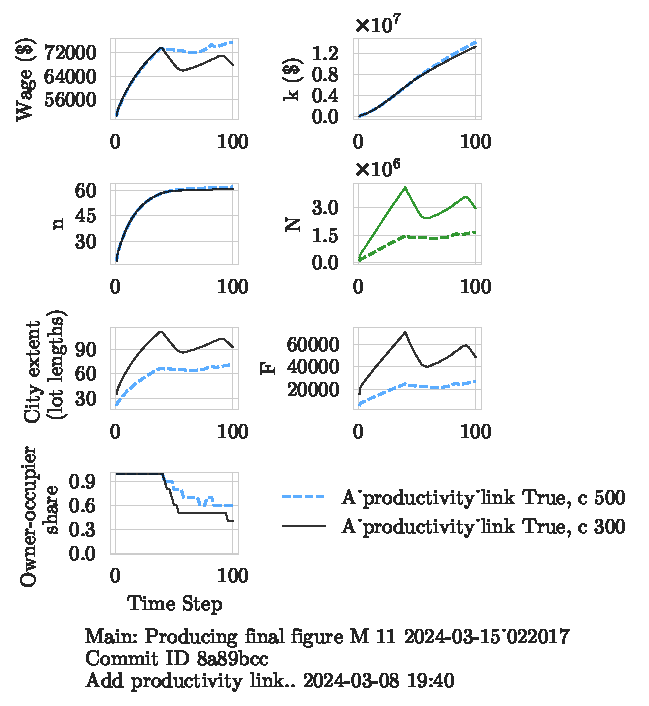
\includegraphics[scale=1, trim={0 1.4cm 0 0},clip]{fig/With-productivity_link-c-15_022017.pdf}
    \caption{The effect of decreasing transportation costs in the presence of productivity impacts}
    \label{fig:Productivity_link_and_c_ownership_trajectory}
\end{figure}

{\color{red} DOES THIS CONTRADICT ITSELF - 1ST AND LAST SENTENCE}

Lower transportation costs also decreases the home-ownership ratio. The reduction in transportation costs leads to an increase in land rents, and the increase in land rents increases the rate of increase of property prices, leading to higher expected capital gains and ultimately owner-occupiers. 

A decline in wage also appears accompany reduced transport costs. This may be understood by noticing that lower transport costs reduce the wage needed to attract workers to the city. 

Lower transportation costs also introduce significant oscillations in population and city size. This is curious, suggesting that we are near an edge of the stability region in the parameter space. CLARIFY?



\newpage
\subsection{Density}
% 'density': [100, 150]
Relaxing restrictions on density should, in theory, affect the ability of people to buy homes. Our results indicate that the effect of density on city population is significant but it has no effect on city extent and no effect on the ownership ratio. The first two results are expected. the third less so but easily explained. Density does not affect transportation cost, and in this test version firm size is not affected. The number of firms rises instead. 

WHAT IS DIFFERENT WITH PRODUCTIFITY. SEEMS TO BE THE SAME AS THE ABOVE.

The share of homeowners is not affected, only the number of homes. Since rent per unit is unchanged at any distance, density alone does not affect the relative advantage of new home buyers and investors, leaving the ratio constant. There are more homes, however, and, since the relative advantages of owners and investors are unchanged, additional homes are distributed the same way.  


\begin{figure}[h!bt]
    \centering
    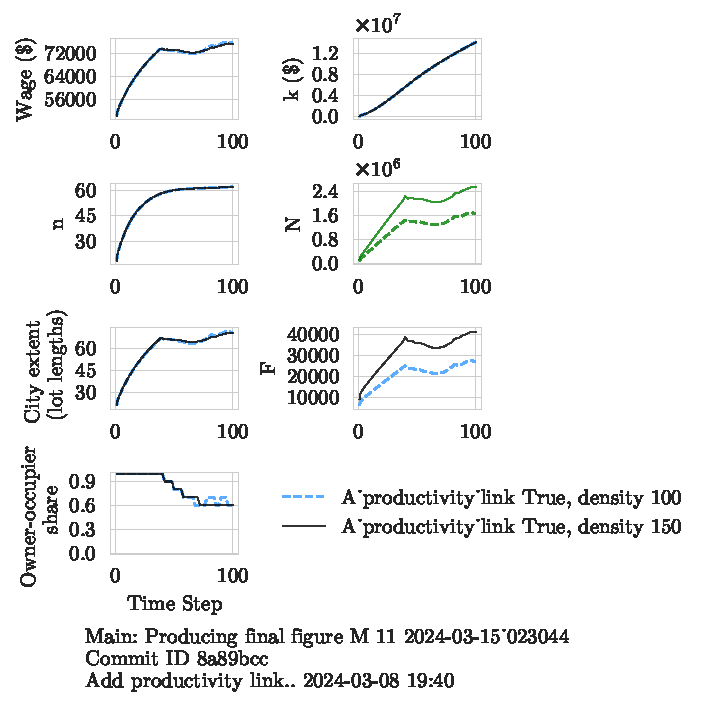
\includegraphics[scale=1, trim={0 1.4cm 0 0},clip]{fig/With-productivity_link-density-023044.pdf}
    \caption{The effect of increasing density in the presence of productivity impacts}
    \label{fig:Productivity_link_and_density_ownership_trajectory}
\end{figure}


\newpage
\subsection{Cost of financing's dependence on borrower's wealth}
{\color{red}In FIGURE ADDDDDDD}, we vary the wealth sensitivity in the presence of a productivity linkage. The higher value is more restrictive:  making it harder for an asset-poor person to get a mortgage. It has no noticeable effect on the ownership ratio. Recall that the purpose of a restrictive policy is to reduce defaults and bankruptcies. The absence of an effect on other variables suggest mortgage assistance is not an effective housing policy.  This is an important result, in our view. {\color{red}DON't REPEAT WHAT YOU SAID IN PREVIOIUS SECIOTN ON THIS, SAY IT'S SAME WITH PODUCTIVITY LINK... ANY NOTABLE RESULTS. }


{\color{red} MAYBE ADD A SUMMARY OF THIS SECTION SAYING THAT THE POLICIES/HOW WE UNDERSTAND THEM SHOULD CHANGE DEPENDING ON WHETHER THERE IS THIS PRODUCTIVITY LINK...}

% 'wealth_sensitivity': [0.15, 0.1, 0.5]

\begin{figure}[h!bt]
    \centering
    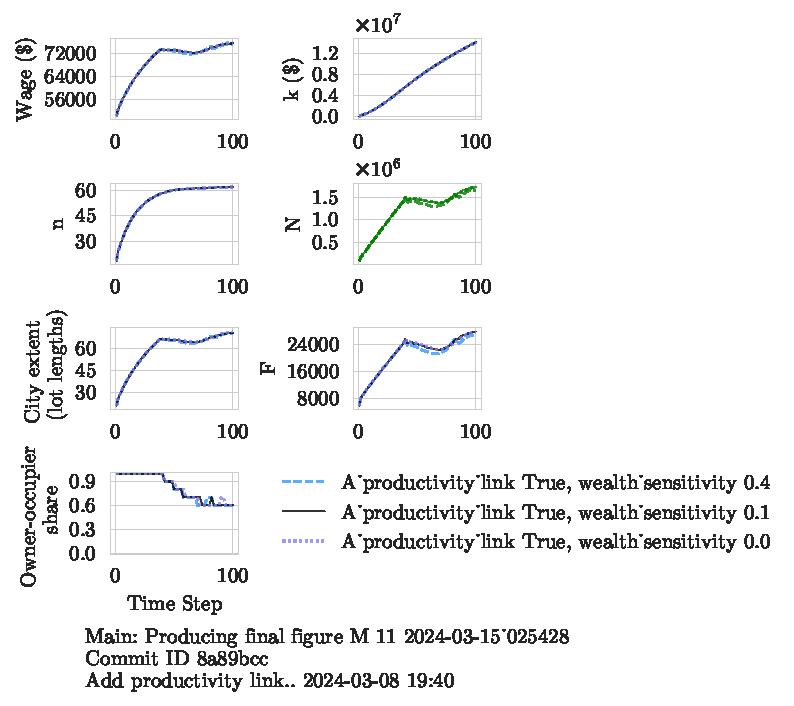
\includegraphics[scale=1, trim={0 1.4cm 0 0},clip]{fig/With-productivity_link-wealth_sensitivity-025428.pdf}
    \caption{The effect of wealth sensitivity of mortgage access in the presence of productivity impacts}
    \label{fig:Productivity_link_and_wealth_sensitivity_ownership_trajectory}
\end{figure}


\newpage
\subsection{The property tax rate}
In the presence of a productivity link, increasing the property tax rate reduces urban size considerably, in contrast to the small effect without the productivity link. This observation suggests that the effect of public sector policies may differ in the presence of a productivity link, and that further investigation of this unrecognized variable should be on the research agenda of urban theorists and policy-makers.

% 'property_tax_rate': [0.1, 0.05, .01] k doing}
% \begin{figure}[h!tb]
%     \centering
%     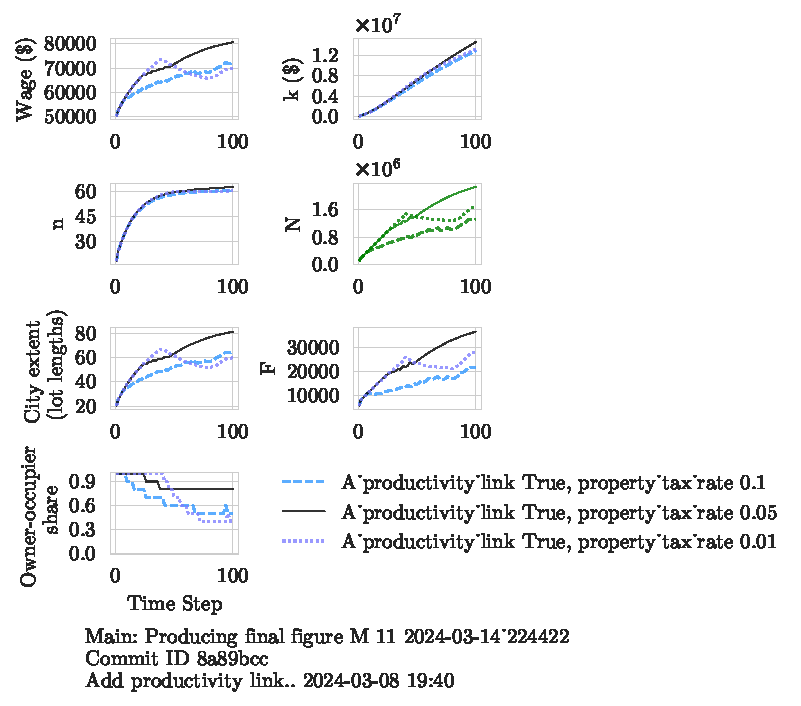
\includegraphics[scale=.8, trim={0 1.4cm 0 0},clip]{fig/With-productivity_link-property_tax-224422.pdf}%  Alternative: 103137.pdf}
%     \caption{The effect of property tax rates in the presence of productivity impacts}
%     \label{fig:Productivity_link_and_property_tax_ownership_trajectory}
% \end{figure}
\begin{figure}[h!tb] 
    \centering
    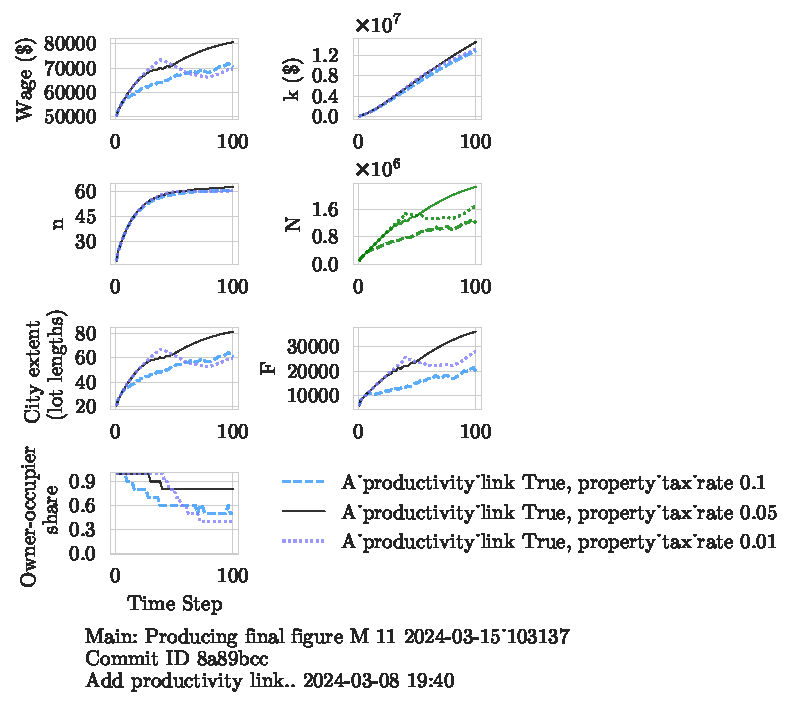
\includegraphics[scale=1, trim={0 1.4cm 0 0},clip]{fig/With-productivity_link-property_tax-103137.pdf}  %224422.pdf}%  Alternative:
    \caption{The effect of property tax rates in the presence of productivity impacts}
    \label{fig:Productivity_link_and_property_tax_ownership_trajectory}
\end{figure}


\newpage
\section{No productivity linkage vs strong productivity linkage }

\subsection{Capital gains taxation on investors}
\begin{figure}[h!tb] 
    \centering
    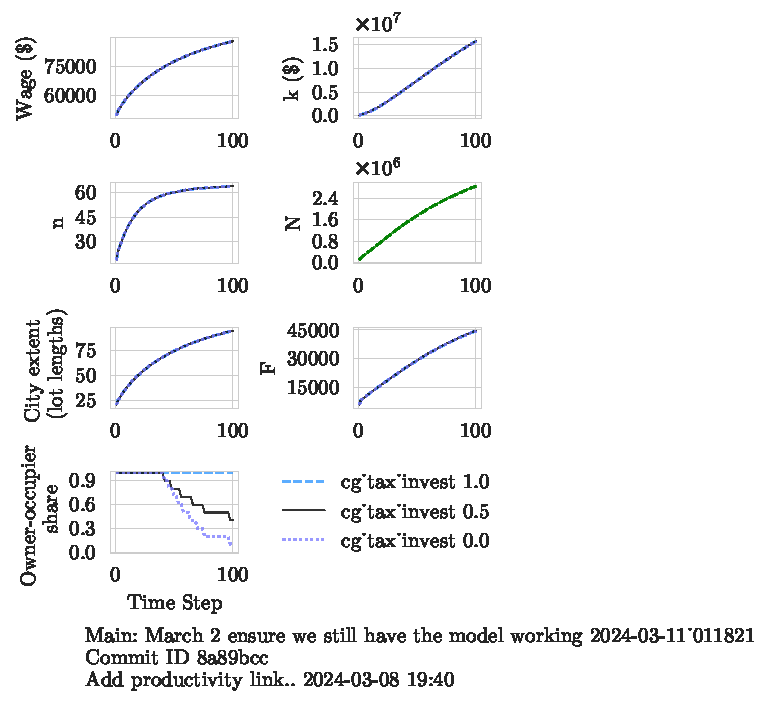
\includegraphics[scale=.75, trim={0 1.4cm 4.5cm 0},clip]{fig/cg_tax_invest-Main-011821.pdf} 
    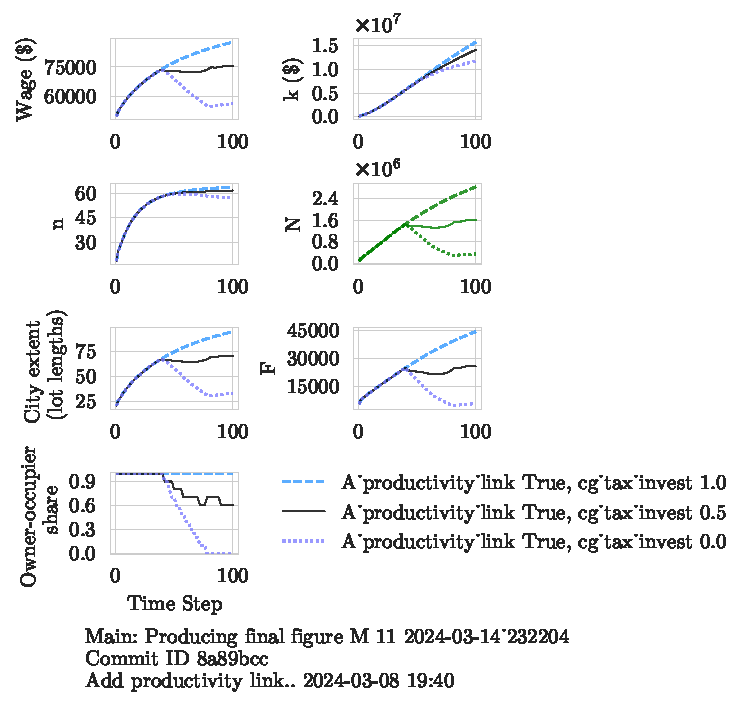
\includegraphics[scale=.75, trim={0 1.4cm 3.7cm 0},clip]{fig/With-productivity_linkcg_tax_invest-232204.pdf} 
    \caption{Capital gains for investors without and with productivity impacts}
    \label{fig:CG-invest_link_W-WO-Cost-of-capital}
\end{figure}
A capital gains tax will in theory reduce investor participation. Figure ~\ref{fig:CG-invest_link_W-WO-Cost-of-capital} shows this is the case without the productivity link. A capital gains tax on housing investment will have a powerful effect.

We have a new result when we introduce the productivity linkage. 
The impact of the tax is larger. This experiment demonstrates that policy parameters are likely to affect the ownership trajectory in different ways when there is a link between financialization and urban productivity and when there is no link.

The dashed line on the left shows a 100\% capital gains tax on land speculation entirely eliminating investor participation in the market, leaving 100\%  owner-occupiers.  Wages are higher the city is larger, and there are more firms. {\color{red} THIS IS BETWEEN WHAT AND WHAT? CLARIFY WHAT YOU ARE COMPARING HERE}

\newpage
\subsection{Capital gains tax on owner occupiers}
\begin{figure}[h!tb] 
    \centering
    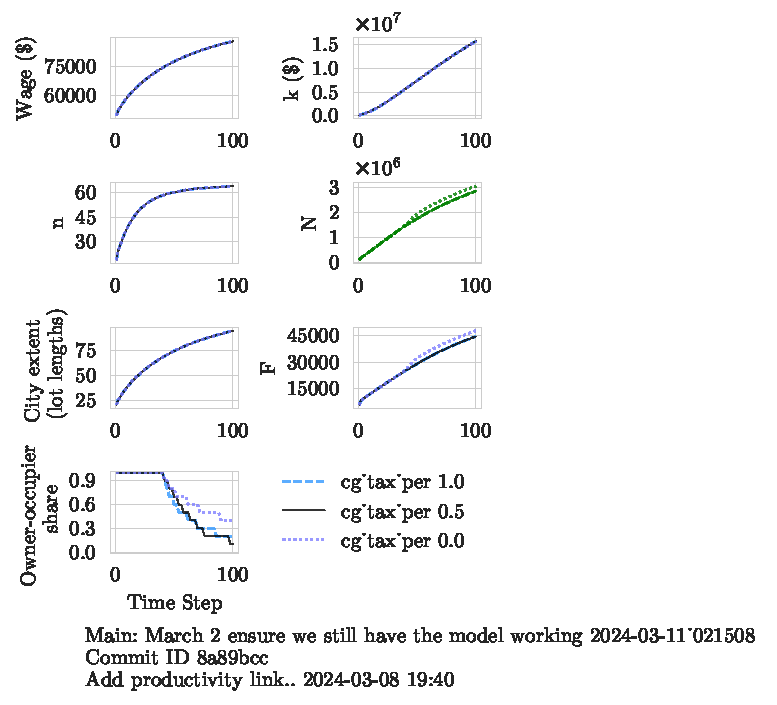
\includegraphics[scale=.75, trim={0 1.4cm 4.5cm 0},clip]{fig/cg_tax_per-Main-021508.pdf} 
    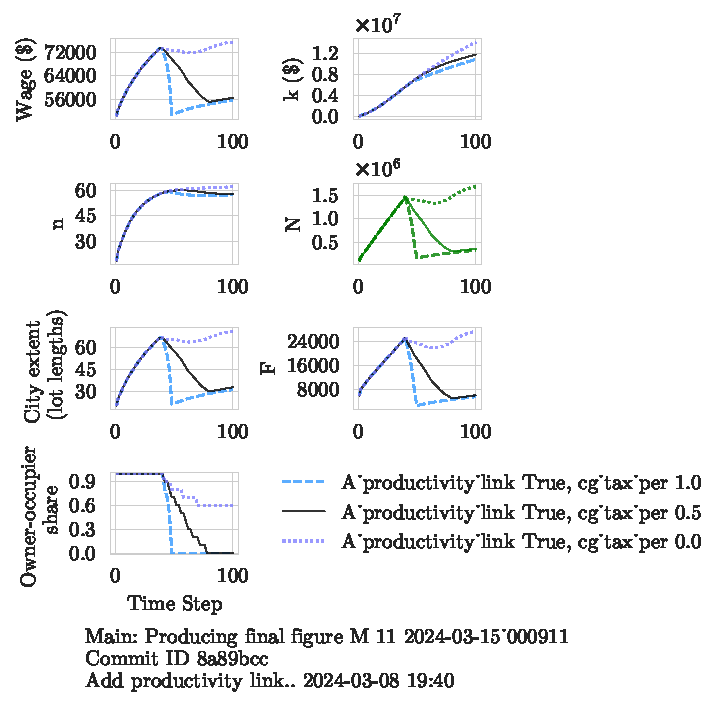
\includegraphics[scale=.75, trim={0 1.4cm 3.5cm 0},clip]{fig/With-productivity_link_cg_tax_per-000911.pdf} 
    \caption{Capital gains for owner occupiers without and with productivity impacts}
    \label{fig:CG-pers_link_W-WO-Cost-of-capital}
\end{figure}

When the capital gains tax on homeowners is higher than the rate of investors, shown by the solid and the dashed lines,  home ownership falls. 

With a productivity link,  When the tax is higher than the rate for investors,  home ownership falls more than in the base case.  Rents will fall for tenants because, with a much lower population and city size, locational rents are lower.

\newpage
\subsection{The cost of capital for investors}
\begin{figure}[h!tb] 
    \centering
    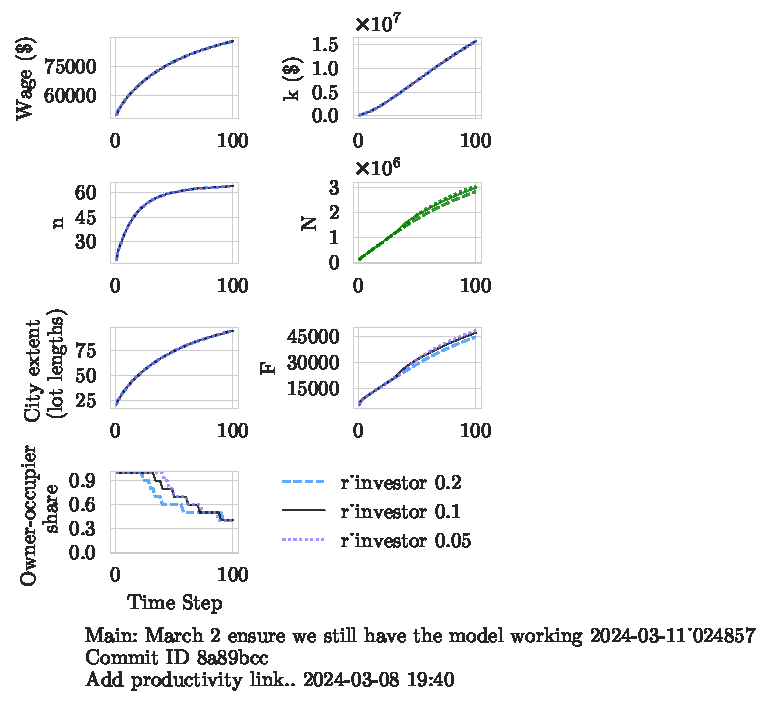
\includegraphics[scale=.75, trim={0 1.4cm 4cm 0},clip]{fig/r_investor-Main-024857.pdf} 
    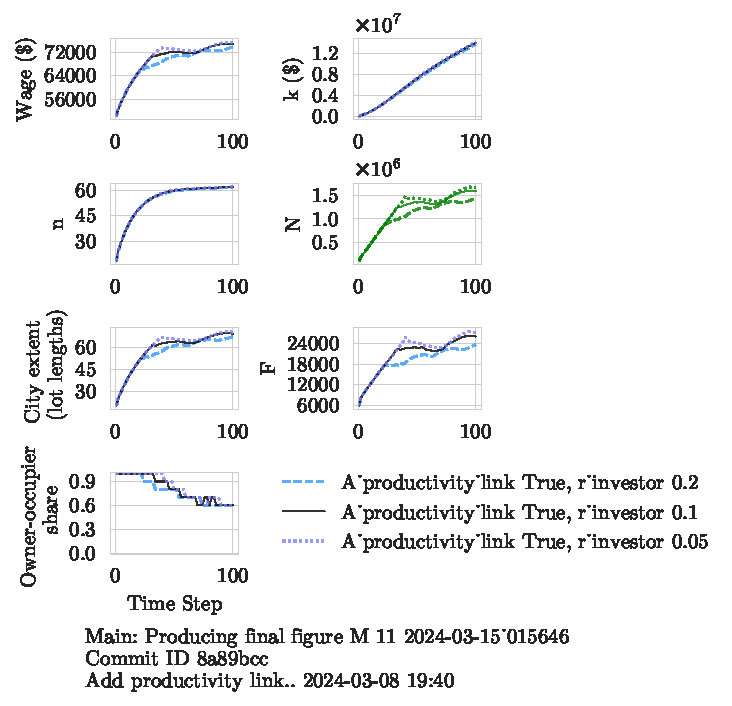
\includegraphics[scale=.75, trim={0 1.4cm 3.5cm 0},clip]{fig/With-productivity_link-r_investor-15_015646.pdf} 
    \caption{Transportation cost without and with productivity impacts}
    \label{fig:Productivity_link_W-WO-Cost-of-capital}
\end{figure}
The cost of capital for investors is not an obvious policy tool, so we don't think this result is of great interest politically, but it warrants further study. Increasing capital costs for investors appears to increase the speed but not the final level of investor ownership.  In addition, it appears to decrease population, suggesting that the cost of acquiring housing rises. 

Even in the presence of strong productivity spillovers, it has little effect, so the cost of capital for investors does not appear to be a promising policy tool.

\newpage
\subsection{Transportation cost}
\begin{figure}[h!tb] 
    \centering
    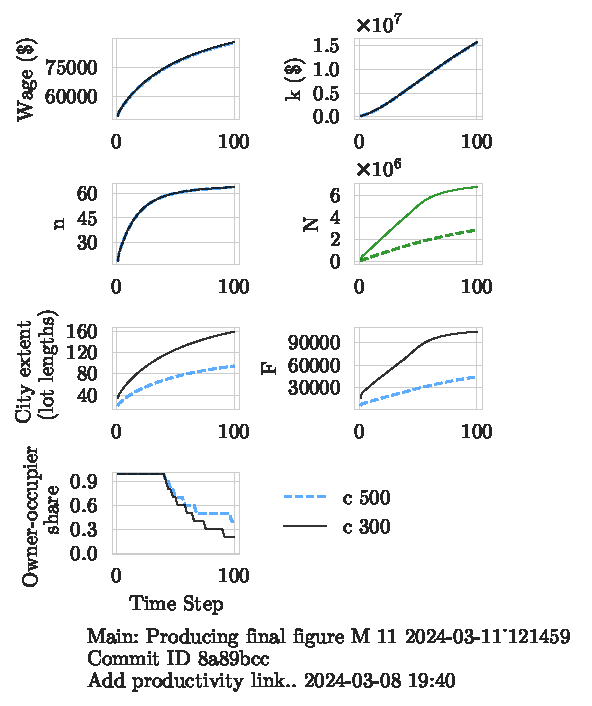
\includegraphics[scale=.75, trim={0 1.4cm 1.5cm 0},clip]{fig/c-Main-121459.pdf} 
    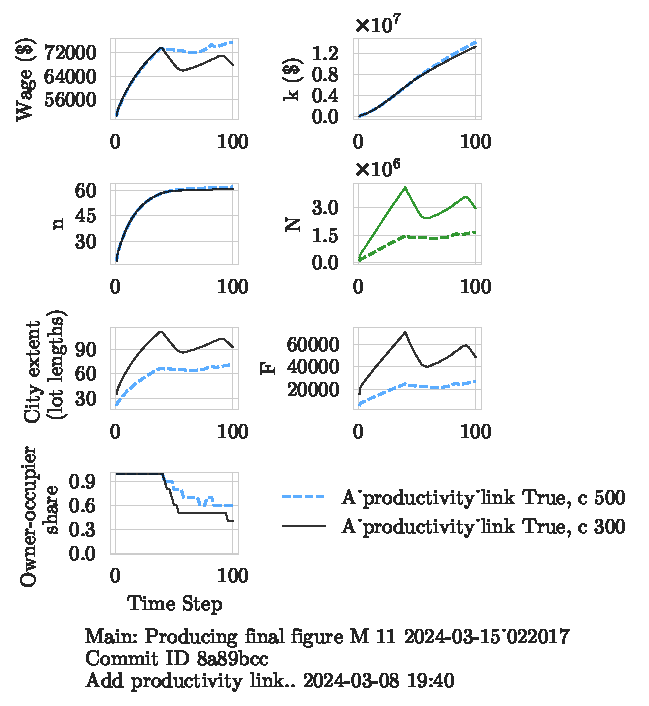
\includegraphics[scale=.75, trim={0 1.4cm 2.3cm 0},clip]{fig/With-productivity_link-c-15_022017.pdf} 
    \caption{Transportation cost without and with productivity impacts}
    \label{fig:Productivity_link_W-WO-transportation-cost}
\end{figure}
Without a productivity link, if we reduce transportation costs for everyone by 40\% the city grows faster and gets larger with lower transportation costs. This effect was indeed observed. 

Less obviously, lower transportation costs also decreased the home-ownership ratio. The reduction in transportation costs leads to an increase in land rents, and the increase in land rents increases the rate of increase of property prices, leading to higher expected capital gains and ultimately less private ownership. 

With productivity links, lower transportation costs also decrease the home-ownership ratio. 
The decline in the wage that appears to accompany reduced transport costs may be understood by noticing that lower transport costs reduce the wage needed to attract workers to the city. 

With productivity links, lower transport costs also introduce significant oscillations in population and city size, which we do not see without the linkage. 



\newpage
\subsection{Density}
\begin{figure}[h!tb] 
    \centering
    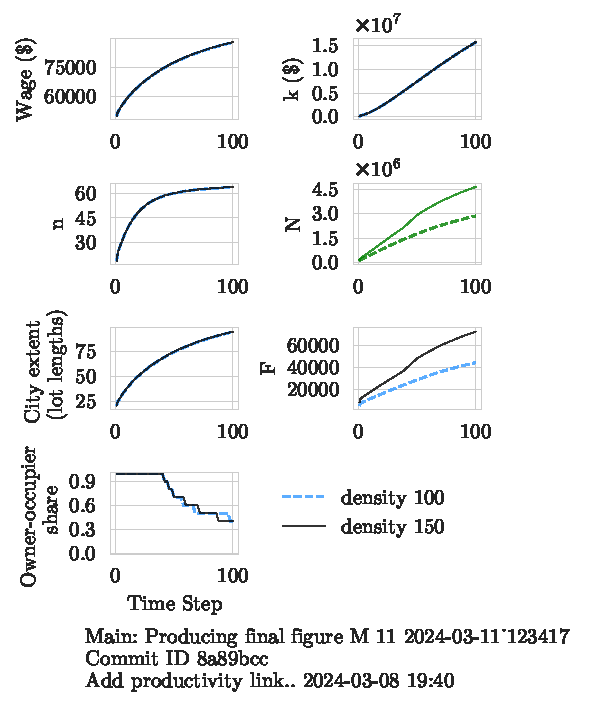
\includegraphics[scale=.75, trim={0 1.4cm 1.5cm 0},clip]{fig/density-Main-123417.pdf} 
    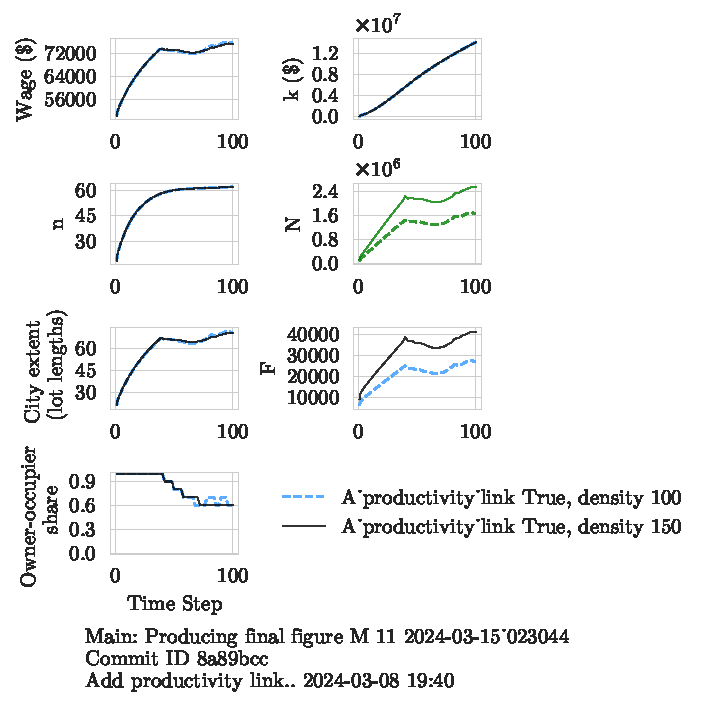
\includegraphics[scale=.75, trim={0 1.4cm 3.2cm 0},clip]{fig/With-productivity_link-density-023044.pdf} 
    \caption{Density without and with productivity impacts}
    \label{fig:Productivity_link_W-WO-density}
\end{figure}
The effect of density on city population is significant but it has no effect on city extent and no effect on the ownership ratio. The share of homeowners is not affected although the number of homes is. 

With productivity links, wages are depressed, and population is lower and appears to cycle.

\newpage %. 
\subsection{Cost of financing's dependence on borrower's wealth}
\begin{figure}[h!tb] 
    \centering
    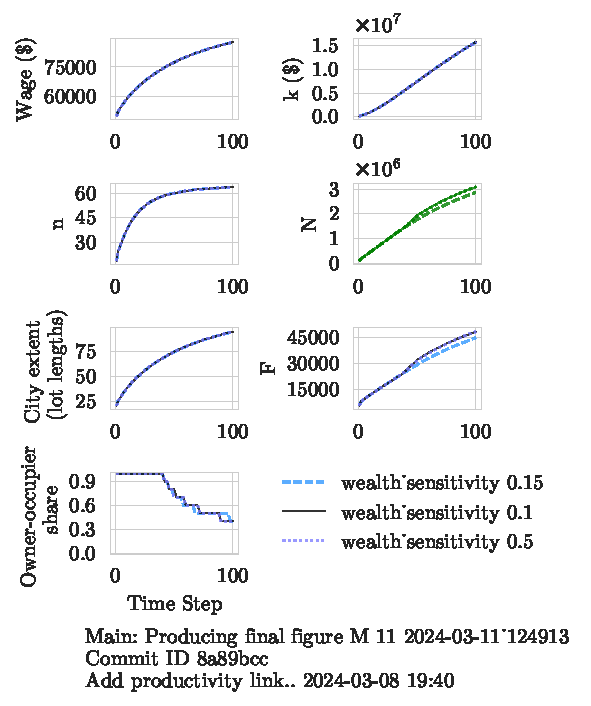
\includegraphics[scale=.75, trim={0 1.4cm 1.0cm 0},clip]{fig/wealth_sensitivity-124913.pdf} 
    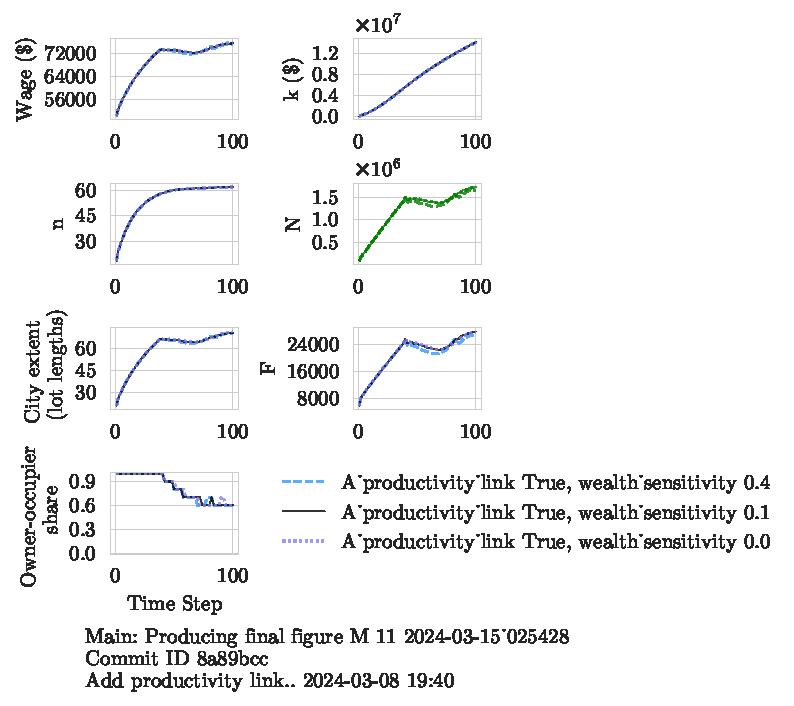
\includegraphics[scale=.75, trim={0 1.4cm 4.75cm 0},clip]{fig/With-productivity_link-wealth_sensitivity-025428.pdf} 
    \caption{Wealth sensitivity rates without and with productivity impacts}
    \label{fig:Productivity_link_W-WO-wealth}
\end{figure}
With and without productivity links, a restrictive mortgage regime slightly reduces the labour supply and city population. It has no noticeable effect on the ownership ratio. The small impact on other variables suggests that mortgage availability can be restricted can be imposed without a significant economic impact on the city. 

In the presence of a productivity linkage, the population is  more variable and is cut roughly in half. Wages are lower, consistent with lower rents.

\newpage
\subsection{The property tax rate}
\begin{figure}[h!tb] 
    \centering
    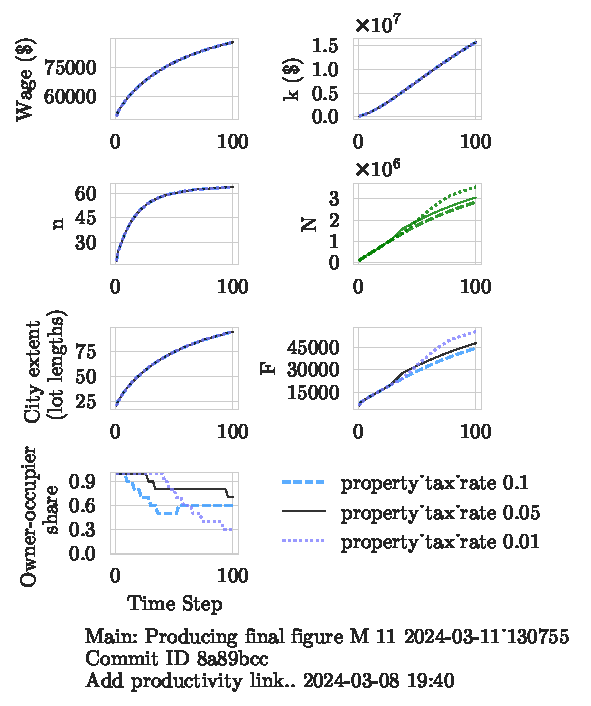
\includegraphics[scale=.75, trim={0 1.4cm .8cm 0},clip]{fig/property_tax_rate-Main-130755.pdf} 
    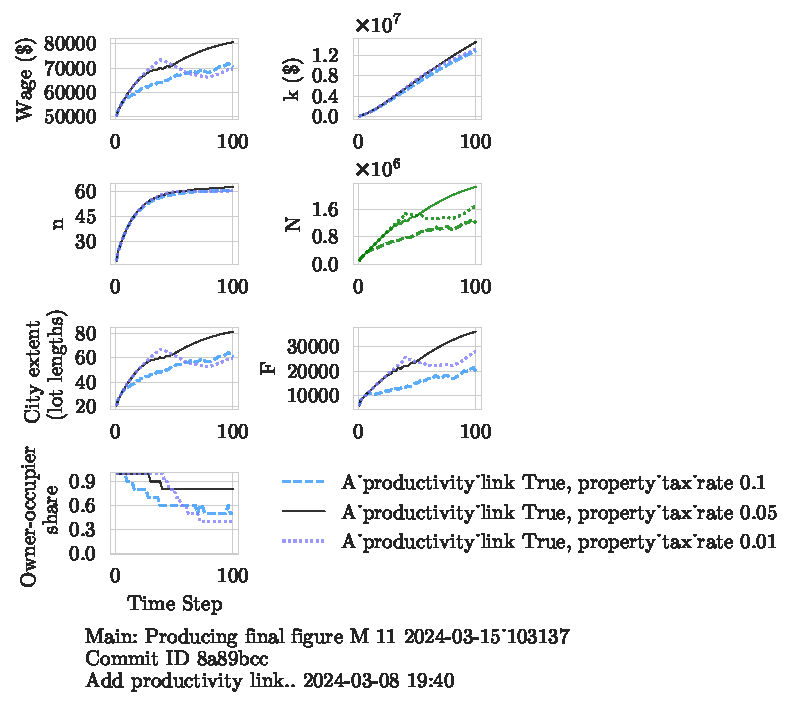
\includegraphics[scale=.75, trim={0 1.4cm 4.75cm 0},clip]{fig/With-productivity_link-property_tax-103137.pdf} 
    \caption{Property tax rates without and with productivity impacts}
    \label{fig:Productivity_link_W-WO-property_tax}
\end{figure}
%no comment on without

In the presence of a productivity link, increasing the property tax rate reduces urban size considerably, in contrast to the small effect without the productivity link. This observation suggests that the effect of public sector policies may differ in the presence of a productivity link, and that further investigation of this unrecognized variable should be on the research agenda of urban theorists and policy-makers.


\begin{figure}[h!tb] 
    \centering
    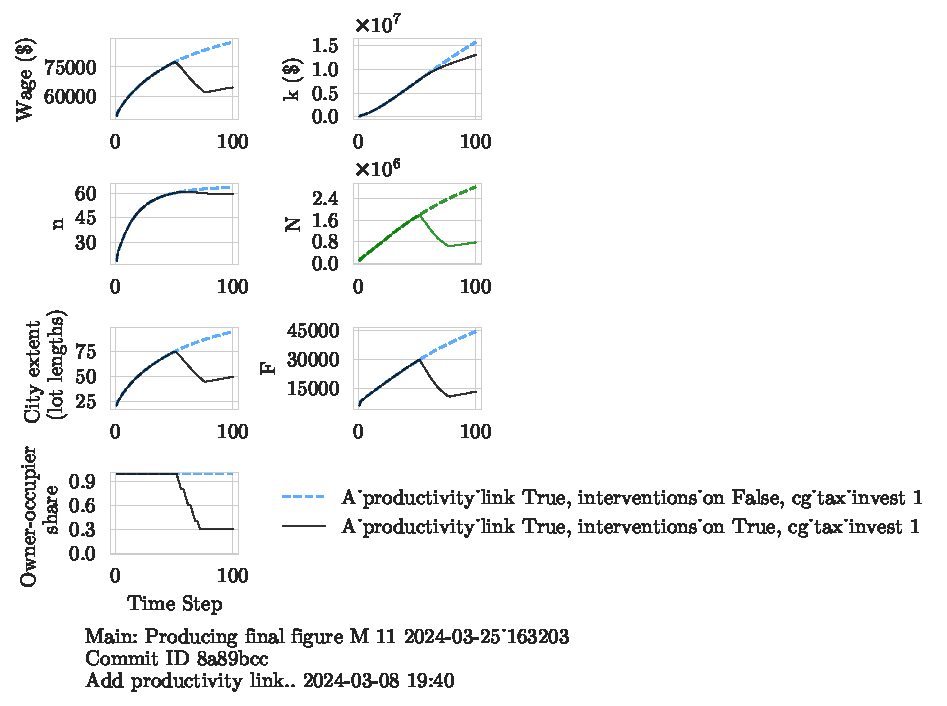
\includegraphics[scale=1., trim={0 1.4cm 7cm 0},clip]{fig/interventions_on-cg_tax_invest-163203.pdf}  %224422.pdf}%  Alternative:
    \caption{Setback resulting from a temporary reduction in the capital gains tax for investors}
    \label{fig:cgtax_setback}
\end{figure}




\section{Illustrating the effect of a transitory policy shock: the capital gains tax for investor}

{\color{red} This is a bit jarring, please explain why you are doing this in, with regards to what you are trying to understand within the thesis. ALSO PLEASE ADD TO INTRO SECTION ABOUT WHAT YOU ARE GOING TO DO IN THIS CHAPTER that you will also do this

MAYBE; Of course, policies are not enacted on fresh systems only. They are introduced at various points. To explore whether policy effects might have different effects base on prior states of the system we consider....}
In this section, we consider a city with a capital gains tax on investors of 100\%, where, after 50 years, the capital gains tax is reduced to zero for 25 years, followed by a return to the original policy.


Following the initial shock, we see a steady decline in wages, some reduction in firm size and capital stock a two-thirds reduction in population and number of firms,  a one-third reduction in city diameter and a 70\% reduction in the owner-occupier share of housing. IN HOW MANY PERIODs??? The city declined to a level approximately were it was at thirty-five periods before the policy change.

When the new policy is reversed, the city returns to a growth rate that is lower than when the policy was implemented. Even after 300 periods it does not return to its original path.



{\color{red} ADD A SUMMARY SAYING THAT THIS SUGGESTS THAT EFFECTS OF POLICY DEPENDS ON WHERE YOU ARE IN A SYSTEM... explain what is suggests }

\section{Summary}
In this Chapter, we have presented and discussed 84 distinct results about policy actions in our model. Forty-two dealt with policy when there is a link between financialization and urban productivity. We believe we are the first to explore this question systematically with a formal simulation model.

Some general observations can be drawn from our results. First, In the absence of linkages between the housing market and the production sector, of the policy tools we consider, only density and transportation cost have much effect. {\color{red} ONE WHAT?? traditional economic measures of urban ??? like ????}



In the presence of linkages, policy tools have much more dramatic effects. This is potentially very important result. 
We did not demonstrate that the link exists, although the literature in our view provides strong indications that there is very likely a linkage.  Our result suggest to us that further research on linkages and how to implement them with models like ours could improve our understanding of the way the urban economy is evolving.   

%we see population effects but no effect on firm variables wage, capital stock or workforce. This is because we force the number of firms to accommodate increases in population. Different assumptions would have allowed growth in both firm size and number, but we were interested in the evolution of population, productivity and ownership rather than the details of the production sector. 

Second, a capital gains tax on speculative investment in housing has a powerful and positive effect with and without a productivity linkage. Without linkage it increases owner occupancy. With a productivity linkage, reducing the capital gains tax reduces the size of the city and wages as well. 

Third, increasing the capital gains tax on owner-occupiers above the level of the capital gains tax on investors has a powerfully negative effect on population and wages.

Fourth, the cost of capital has surprisingly little effect on any variables in either case.

Fifth, Transportation cost has a strong effect, but that result is entirely expected. Unexpected and warranting further investigation is that low transportation costs with financial system spillovers appears to induce something like cyclical behaviour.

Sixth, increasing density increases the population, as expected, but does not affect wages or city extent 
{\color{red} or ownership ratios.}

Seventh, a more restrictive mortgage market does not affect the production sect3or or city size.

Eighth, increasing property taxes reduced the number of owner occupiers, but has only a small effect on city size when there is no linkage. to financialization but depresses wages population and city size when there is a linkage. 


{\color{red} ADD A SUMMARY saying that this provides useful information about .... and suggests that WHICH in particular would be useful to study further. AND say that also studying shifts mid=trajectory would be useful as the shock thing suggests.

PROBABLY REFERENCE PHRASING FROM INTRO: 
The resulting model suggests two basic hypotheses:
\begin{enumerate}
    \item Financialization of the housing market will result in the tenantization of the urban middle class as financial capital acquires more of the housing stock. % vs decline of the urban middle class
    \item Financialization of the housing market will result in reduced growth of urban productivity as the flow of rents is diverted from real investment to the financial sector.
\end{enumerate} }



